\begin{paper}{1}
\begin{header}
\title{On the quantum mechanics of electrons in crystal lattices}
\author{Felix Bloch}
\location{Leipzig}
\note{Received August \Nth{10}, 1928.}
\makeheader
\end{header}

\newcommand{\mfa}{\mathfrak{a}}
\newcommand{\mfb}{\mathfrak{b}}
\newcommand{\mfc}{\mathfrak{c}}
\newcommand{\mfr}{\mathfrak{r}}

\begin{abstract}
The motion of an electron in the lattice is investigated by \?{schematizing}{schematisieren} this through an initially strictly doubly-periodic force field. Taking into account the Fermi statistics of the electrons allows our model to make statements about the portion of the lattice's specific heat arising from them. Further, it is shown that taking into account the thermal lattice vibrations provides the order of magnitude and temperature dependence of the electrical conductivity of metals in qualitative agreement with experiment.
\end{abstract}

\section*{Introduction.} The electron theory of metals has shown progress for some time, based upon the application of quantum theoretical principles to the electron gas. First Pauli\footnote{W. Pauli, ZS. f. Phys. 41, 81, 1927.}, under the assumption that the metals' electrons are able to move completely freely in the lattice and obey the Fermi\footnote{E. Fermi, ibid 36, 902, 1926.} statistics, was able to explain the temperature-independent paramagnetism of the alkalines. The electrical and thermal properties of the electron gas were then more closely investigated by Sommerfeld, Houston and Eckart\footnote{A. Sommerfeld, W.V. Houston, C. Eckart, ibid 47, 1, 1928.}. The fact of free conduction electrons is considered by them as given and their interaction with the lattice is only taken into account as a first phenomologically-introduced, then a rigorously founded (by Houston\footnote{W.V. Houston, ibid 48, 449, 1928.}) mean free path. Finally, Heisenberg\footnote{W. Heisenberg, ibid 49, 619, 1928.} has shown that in the other limiting case where the electrons are thought of as bound to the ions in the lattice, and the exchange processes among them are only taken into account in the next approximation, where the intermolecular field that is decisive for ferromagnetism finds its explanation. 

Here the intermediate standpoint between the two above-mentioned treatments will be taken insofar as the exchange of electrons remains unaccounted for, on the other hand they are not considered to be freely moving, but rather in a force field that has the same periodicity as the lattice itself. From this assumption it shall be shown how and to what extent the fact of free conduction electrons can be quantum-mechanically justified. Essentially, the distinction stressed by Hund\footnote{F. Hund, ZS. f. Phys. 40, 742, 1927.} as against the classical mechanics, that it is impossible to hold an electron fixed in a potential well, however deep.  So long as one assumes a strictly periodic force field, on the contrary each of the $N$ electrons can pass through the lattice unhindered. Only deviations from the periodicity as a consequence of the thermal motion of the atoms gives rise to a finite mean free path and conductivity.

\section{The quantum mechanics of an electron in a triply-periodic force field.}
According to Schr\"odinger the time-independent probability amplitude $\psi(xyz)$ associated with the energy $E$ obeys the differential equation
\nequ{1}{
\Delta\psi + \mu(E-V)\psi = 0 \quad
\mu = \frac{8\pi^2 m}{h^2}
}

$V$ is the electrostatic potential in which the electron has to move in the lattice. We make the following assumption about its dependence on the coordinates $x,y,z$:

Putting the origin of the coordinates in the lattice and letting $\mfa,\mfb,\mfc$ be the basis vectors of the lattice, so that the position vector of any lattice point is given by
\uequ{
\mfr_G = g_1\mfa + g_2\mfb + g_3\mfc, \quad \text{$g_1 g_2 g_3$ = integers,}
}
then $V$ satisfies the periodicity condition
\nequ{2}{
V(\mfr) = V(\mfr + g_1\mfa + g_2\mfb + g_3\mfc),
}
where $g_1g_2g_3$ again denote any integers and the position vector $\mfr$ is placed at the position of the triplet $x,y,z$.

The question as to the eigenvalues and the eigensolutions of the differential equations now depends on the boundary conditions which the latter are to obey. The most convenient condition would be the vanishing of $\psi$ at the boundary surfaces of the crystal, since the probability that the electron is found outside apparently practically vanishes.

However, this would single out the boundary surfaces, which would complicate the treatment, and obviously has nothing to do with the physical nature of the problem. The fact is completely analogous to that met previously in the theory of specific heats of crystal lattices. The difficulty was lifted at the time by Born and K\'arm\'an\footnote{M. Born and Th. v. K\'arm\'an, Phys. ZS. 13, 297, 1912; 14, 15, 1918.} by introducing the cyclic condition that the elastic \?{normal modes}{Eigenschwingungen} should exhibit a threefold spatial periodicity, and it is convenient to put the same requirement for the probability amplitudes in the lattice electrons. This means that not only the elastic properties, but also the properties arising from the electrons of \?{the whole}{des ganzen, noch so gro{\SS}en} lattice are known as soon as they are known in a sufficiently large partial region -- say, the parallelepiped spanned by the vectors $G_1\mfa,G_2\mfb,G_3\mfc$, where $G_1G_2G_3$ are large integers. \?{The whole lattice emerges from this base region and its properties through  periodic repetitions}{Das Gesamtgitter geht aus diesem Grundgebiet mitsamt seinen Eigenschaften durch periodische Wiederholung hervor}; the identical ways of treating "$\psi$-waves" and elastic waves will prove advantageous as soon as we have to investigate their interaction, as will actually be the case for the problem of resistance (\S5).

That something can already be said about the solutions of (1) on the grounds of the periodicity (2) of the potential alone, is suggested by the group-theoretical investigations that Wigner\footnote{E. Wigner, ZS. f. Phys. 43, 624, 1927.} first applied to quantum mechanical questions. We repeat his findings to the extent that they are needed here.

For simplicity we will assume that the lattice vectors $\mfa,\mfb,\mfc$ are perpendicular to one another, and the coordinate axes lie in their directions; but the following considerations also suffice for an arbitrary triclinic crystal.

Let
\uequ{
|\mfa|=a, \quad |\mfb|=b, \quad |\mfc|=c,
}
so that the three substitutions
\nequ{3}{
\begin{array}{rlll}
	R: & x'=x+a, & y'=y, & z'=z\\
	S: & x'=x, & y'=y+b, & z'=z\\
	T: & x'=x, & y'=y, & z'=z+c
\end{array}
}
belong to the substitution groups of the differential equation (1), i.e. along with each solution $\psi(x\,y\,z)$,$\psi(x'y'z')$ is also a solution. Now let $\psi_1(d\,y\,z\,E) \psi_2(x\,y\,z\,E), \dots, \psi_i(x\,y\,z\,E)$ be a set of linearly-independent eigenfunctions of (1) which belong to the eigenvalue $E$ and from which each solution associated to $E$ can be formed. Then
\nequ{4}{
\psi_\lambda(x+a, y, z, E) &= \sum\limits_{\varx=1}^l a_{\varx\lambda}\psi_\varx(x\,y\,z, E),\\
\psi_\lambda(x, y+b, z, E) &= \sum\limits_{\varx=1}^l b_{\varx\lambda}\psi_\varx(x\,y\,z, E),\\
\psi_\lambda(x, y, z+c, E) &= \sum\limits_{\varx=1}^l c_{\varx\lambda}\psi_\varx(x\,y\,z, E),\\
}
That means that the group elements $R,S,T$ are "represented" by the respective matrices $(a_{\varx\lambda}), (b_{\varx\lambda}), (c_{\varx\lambda})$. Similarly the representation of any product $R^{g_1} S^{g_2} T^{g_3}$, i.e. the substitution obtained if one applies one after another $R$ $g_1$ times, $S$ $g_2$ times, $T$ $g_3$ times, can be found in the corresponding matrix product $(a_{\varx\lambda})^{g_1}(b_{\varx\lambda})^{g_2}(c_{\varx\lambda})^{g_3}$. But now the functions should be $\psi_\varx(x\,y\,z\,E)$ ($\varx=1,2,\dots,l$), since as eigenfunctions of our problem with the above-discussed boundary condition of a threefold spatial periodicity with periods $G_1a, G_2b, G_3c$, they are carried over into themselves by the substitutions $R^{G_1},S^{G_2},T^{G_3}$. This means, for the representation by matrices:
\nequ{5}{
(a_{\varx\lambda})^{G_1} = (b_{\varx\lambda})^{G_2} = 
(c_{\varx\lambda})^{G_3} = \delta_{\varx\lambda},
}
where $\delta_{\varx\lambda}$ denotes the unit matrix. The substitution group characteristic for our problem is then the direct product of three cyclic groups that \?{commute with one another}{miteinander vertauschbarer}\footnote{Cf Speiser, Theory of Groups of Finite Order, 2nd edition, p.16.} of respective order $G_1,G_2,G_3$. The simplest, the irreducible representation obtained if one starts with, instead of the $\psi_\varx$, another system of linearly independent eigenfunctions
\uequ{
\psi_\lambda' = \sum\limits_{\varx=1}^l t_{\varx\lambda}\psi_\varx
\quad \text{$\lambda=1,2,\dots,l$}
}
and chooses the matrix $(t_{\varx\lambda})=t$ so that
\uequ{
(a_{\varx\lambda}') = t^{-1}(a_{\varx\lambda})t;\quad
(b_{\varx\lambda}') = t^{-1}(b_{\varx\lambda})t;\quad
(c_{\varx\lambda}') = t^{-1}(c_{\varx\lambda})t
}
are diagonal matrices.

This is always possible according to well-known rules, since the matrices $(a_{\varx\lambda}), (b_{\varx\lambda}), (c_{\varx\lambda})$ commute with one another. Now from (5) it will follow that
\nequ{5'}{
(a_{\varx\lambda}')^{G_1} =
(b_{\varx\lambda}')^{G_2} =
(c_{\varx\lambda}')^{G_3} = \delta_{\varx\lambda}.
}
The diagonal elements of $(a_{\varx\lambda}')^{G_1}, (b_{\varx\lambda}')^{G_2}, (c_{\varx\lambda}')^{G_3}$ are then roots of unity, i.e. we can write
\nequ{5''}{
a_{\lambda\lambda}' = \exp{\frac{2\pi i}{G_1}k_\lambda},
b_{\lambda\lambda}' = \exp{\frac{2\pi i}{G_2}l_\lambda},
c_{\lambda\lambda}' = \exp{\frac{2\pi i}{G_3}m_\lambda},
}
where $k_\lambda,k_\lambda,l_\lambda$ are integers, and from (4) we have
\nequ{4'}{
\psi_\lambda'(x+a,y,z,E)&=\sum\limits_\varx a_{\varx\lambda}'\psi_\varx'(xyzE) = a_{\lambda\lambda}'\psi_\lambda'(xyzE)
= \exp{\frac{2\pi i}{G_1}k_\lambda}\psi_\lambda'(xyzE),\\
\psi_\lambda'(x,y+b,z,E)&=\sum\limits_\varx b_{\varx\lambda}'\psi_\varx'(xyzE) = b_{\lambda\lambda}'\psi_\lambda'(xyzE)
= \exp{\frac{2\pi i}{G_2}l_\lambda}\psi_\lambda'(xyzE),\\
\psi_\lambda'(x,y,z+c,E)&=\sum\limits_\varx c_{\varx\lambda}'\psi_\varx'(xyzE) = c_{\lambda\lambda}'\psi_\lambda'(xyzE)
= \exp{\frac{2\pi i}{G_3}m_\lambda}\psi_\lambda'(xyzE).
}
To each eigenvalue is associated a completely determined \?{system of numbers}{Zahlensystem} $k_\lambda,l_\lambda,m_\lambda$.

The relations (4') for the eigenfunctions $\psi_\lambda'$ are completely equivalent with the statement: every eigenfunction can be represented in the form
\nequ{6}{
\psi_{klm}(xyz) = \exp{2\pi i\left(\frac{kx}{aG_1} + \frac{ly}{bG_2} + \frac{mz}{cG_3}\right)}\cdot u_{klm}(xyz),
}
where $u_{klm}$ is a triply periodic function with periods $a,b,c$ and $k,l,m$ denote integers. If we introduce the lengths of the vectors spanning the base parallelepiped
\uequ{
aG_1 = K,\quad
bG_2 = L,\quad
cG_3 = M,
}
then from (6)
\nequ{6a}{
\psi_{klm} = \exp{2\pi i\left(\frac{kx}{K} + \frac{ly}{L} + \frac{mz}{M}\right)}\cdot u_{klm}(xyz).
}

Nothing is said about the specific form of the function $u_{klm}$. This naturally depends on how the potential flows in individual cases, and additionally it could very well depend on quantum numbers outside of the $k,l,m$.

The fact that according to (6a) a factor of $\exp{2\pi i\left(\frac{kx}{K}+\frac{ly}{L}+\frac{mz}{M}\right)}$ can always be split off from the eigenfunctions, where the rest onlt exhibits the periodicity of the lattice, can be intuitively formulated so that it involves plane de Broglie waves \?{which are modulated in the rhythm of the lattice structure}{die im Rhythmus des Gitteraufbaus moluliert sind}.\footnote{Added during editing. As I unfortunately only noticed subsequently, E.E. Wittmer and L. Rosemfeld, ZS. f. Phys. 48, 530, 1928 have already derived the same result in other ways.}

This similarity with the eigenfunctions of the force-free motion is what gives the lattice electrons the mobility essential to electrical conduction. In order to show this, we form the expression, which according to Schr\"odinger\footnote{E. Schr\"odinger, Ann d. Phys, (4) 81, 138, 1926.} specifies the total current in the $x$-direction of the state $k,l,m$ of an electron:
\nequ{7}{
s_{klm}^x = \frac{eh}{4\pi im}\int\left(\overline{\psi}_{klm}\pX{\psi_{klm}}\pY{x} - \psi_{klm}\pX{\overline{\psi}_{klm}}\pY{x}\right)\d\tau.
}

The integration stretches over the whole base parallelepiped and the eigenfunctions (6a) are orthogonal and normalized in this region. The expression (7) can be recast as follows: According to (1)
\uequ{
\overline{\psi}\Delta\psi - \psi\Delta\overline{\psi} = 0.
}
So according to the Green Theorem
\uequ{
\int x\left(\overline\psi\Delta\psi - \psi\Delta\overline\psi \right)\d\tau + 
\int x\left[\left(\grad\psi, \grad\overline\psi \right) - \grad\overline\psi, \grad\psi\right]\d\tau\\
 = -\int{\left(\overline\psi\pX\psi\pY{x} - \psi\pX{\overline\psi}\pY{x}\right)}\d\tau + 
 \int{x\left(\overline\psi\pX\psi\pY{n} - \psi\pX{\overline\psi}\pY{n}\right)}\d{f} = 0,
}
where the last integral is taken over the whole surface of the base parallelepiped and $\pX{}\pY{n}$ denotes differentiation with respect to the normals. Now because of the periodicity the expressions $\overline\psi\pX\psi\pY{n}$ and $\psi\pX{\overline\psi}\pY{n}$ are always equal and opposite at corresponding points of the surface, so that only the $x$-side surface contributes anything, and what remains is
\nequ{8}{
s_{klm}^x &= \frac{eh}{4\pi im}\int\left(\overline\psi_{klm}\pX{\psi_{klm}}\pY{x} - \psi_{klm}\pX{\overline\psi_{klm}}\pY{x}\right)\d\tau\\
 &= K\frac{eh}{4\pi im}\int\left(\overline\psi_{klm}\pX{\psi_{klm}}\pY{x} - \psi_{klm}\pX{\overline\psi_{klm}}\pY{x}\right)\d{f},
}
where the integral is only over the right-side surface. The proportionality with $K$ is only apparent, since the normalization of $\psi_{klm}$ must be taken into account. Now (8) in general does not vanish at all, so that the state $k,l,m$ actually corresponds to a mean momentum, i.e. a forward motion.

Our up to now general considerations shall now be illustrated with two limiting cases, those of the completely free and the very firmly bound electrons. I nature of course one always finds something between the two.

First the free electrons. Here, because of normalization, from (6a)
\uequ{
\psi_{klm} = \frac{1}{\sqrt{KLM}}\exp{2\pi i\left(\frac{kx}{K} + \frac{ly}{L} + \frac{mz}{M}\right)},
}
i.e. our quasi-plane de Broglie waves (6a) actually go over in this limiting case to the well-known de Broglie waves. Here from (8)
\nequ{9}{
s_{klm}^x = \frac{e}{m}\frac{kh}{K},
}
where $\frac{kh}{K}$ represents in the known fashion the momentum associated to the wavelength $\frac{K}{k}$. The usual translational motion is here associated in a totally natural way with the Hund \?{position exchange}{Platzwechsel} of the electrons in equal potential wells.

As the ideal case opposite to the completely free electrons shall be extensively discussed \WTF{no punctuation, section 2 just starts}

\section{The limiting case of strongly bound electrons.}
This is represented by a potential $V$, which is very negative in the immediate surroundings of each lattice point, though strongly increases at distances on the order of half a lattice constant. At these points, as Hund has shown\footnote{loc cit}, the eigenfunctions, as well as their derivatives, will be very small. Now in order to see how the \?{conductivity}{Leitercharakter} of a lattice depends on the binding strengths of the electrons, one need only put the right-side surface of the base parallelepiped in between two neighboring lattice planes in (8). (Because the current is divergenceless, the expression (8) is naturally independent of the specific position of the surface!) They then run exclusively at points of high potential, so that there the quantities $\psi$ and $\pX\psi\pY{x}$ and with them the current become very small and vanishes in the limiting case of infinitely strongly-bound electrons (ideal insulators).

A more precise picture of our model is obtained by interpreting the differential equation (1) as a perturbation problem in a similar manner  as Heitler and London\footnote{W. Heitler and F. London, ZS. f. Phys. 44, 455, 1927.} did for the case of two hydrogen atoms. While there it dealt with a two-body problem, here as a consequence of ignoring electron interactions it only appears as a one-body problem. There the infinitely strong binding will be considered as the unperturbed starting point.

Next we represent the potential of (1) as a sum of the potentials arising from the different lattice points. Here it should be noted that what is decisive here is not only the field arising from the metal ions, but the leftover conduction electrons also provide a contribution. One can also think of it as being brought about by the continuous \?{cloud of charge}{Ladungswolke} arising from them\footnote{Cf e.g. E. Fermi, ZS. f. Phys. 48, 73, 1927.}; however their influence in the immediate surroundings of an atom is small, so that it will be justified to simply set the potential arising from the individual lattice points to that of the ions.

If the ion at the lattice point
\uequ{
\mfr_{g_1g_2g_3} = g_1\mfa + g_2\mfb + g_3\mfc,
}
then let its potential be given by
\uequ{
U_{g_1g_2g_3}(xyz) = U(x-g_1a,y-g_2b,z-g_3c),
}
and
\nequ{10}{
V(xyz) = \sum\limits_{g_1g_2g_3 = -\infty}^{+\infty}U_{g_1g_2g_3}(xyz).
}
Now if we consider the differential equation
\nequ{11}{
\Delta\varphi_{g_1g_2g_3} + \mu(E-U_{g_1g_2g_3})\varphi_{g_1g_2g_3}=0,
}
which apparently corresponds to the motion of an electron about an isolated ion of the metal lattice. Those of our real (vanishing at infinity) eigensolutions associated with the lowest eigenvalue $E_0$ are
\nequ{12}{
\varphi_{g_1g_2g_3}(xyz) = \varphi(x-g_1a, y-g_2b, z-g_3c).
}

As long as the effect of the metal ions on their neighbors is ignored, our system's degree of degeneracy is the same as there are ions in the lattice, since the same energy $E_0$ is associated with the motion (11) about each of the ions. Accordingly we make the \textit{Ansatz}
\nequ{13}{
E=E_0+\varepsilon\quad
\psi = \sum\limits_{g_1g_2g_3}a_{g_1g_2g_3}\varphi_{g_1g_2g_3} + v
}
for the solution of (1), where $\varepsilon$ and $v$ are to be small quantities, whose products and higher powers are to be ignored. Then from (1), using (11)
\nequ{14}{
\Delta v + \mu(E_0-V)v = -\mu\sum\limits_{g_1g_2g_3}\varphi_{g_1g_2g_3}(\varepsilon - V + U_{g_1g_2g_3}).
}

So for this equation, inhomogenous in $v$, to have a solution at all, it is well known that the right side must be perpendicular to the solutions of the homogenous solutions. Now though we do not know the latter, they will differ less from the solutions $\varphi_{g_1g_2g_3}$ of (11) the smaller the interaction of the neighboring atoms is. So instead of actual orthogonality we require\footnote{The procedure is completely analogous to that applied by Heitler and London, loc cit.}
\nequ{15}{
\sum\limits_{g_1g_2g_3} a_{g_1g_2g_3}\int(\varepsilon - U'_{g_1g_2g_3})\varphi_{g_1g_2g_3}\varphi_{h_1h_2h_3}\d\tau = 0
}
where
\uequ{
h_1h_2h_3=-\infty\dots + \infty\\
U'_{g_1g_2g_3} = V-U_{g_1g_2g_3}
}
and the integral is over the whole space.

We now make the following assumption about the potential $U(xyz)$ around an isolated ion, which is justified by our choice of (11) as the unperturbed starting point of the problem. $U$ shall be negative infinity at the point $x=y=z=0$, vanish at infinity, and is already very small at distances from the zero point of the order of half the lattice constant.

Then the eigenfunctions $\varphi_{g_1g_2g_3}$ are only significantly different from zero in the immediate vicinity of the point $(g_1\,g_2\,g_3)$, and if we still consider them as normalized, then up to terms of the order of $v$ we can set
\nequ{16}{
\psi\varphi_{g_1g_2g_3}\varphi_{h_1h_2h_3}\d\tau = \begin{cases}
 	1 & \text{if $g_1=h_1,g_2=h_2,g_3=h_3$,}\\
 	0 & \text{in all remaining cases.}
 \end{cases}
}

In the second integral occurring in (15)
\uequ{
J=\int U'_{g_1g_2g_3}\varphi_{g_1g_2g_3}\varphi_{h_1h_2h_3}\d\tau,
}
it is to be imagined that $U'_{g_1g_2g_3}$ almost vanishes in the vicinity of the point $(g_1\,g_2\,g_3)$, namely is equal to the sum of the potentials produced there by the remaining lattice points. For this reason, in forming $J$ we must also consider the case where the triplet $(h_1\,h_2\,h_3)$ denotes a lattice point neighboring $(g_1\,g_,g_3)$. Those further away need not be considered, since there the value of $\varphi_{g_1g_2g_3}$ has already become too small. We will assume in the following that we are dealing with a simple cubic lattice and that the functions $U(xyz)$ and $\varphi(xyz)$ are spherically symmetrical. Then we will have to set
\nequ{17}{
\int U'_{g_1g_2g_3}\varphi_{g_1g_2g_3}\varphi_{h_1h_2h_3}\d\tau = \begin{cases}
 	\alpha & \text{if $(h_1\,h_2\,h_3)=(g_1\,g_2\,g_3)$,}\\
 	\beta &  \text{if $(h_1\,h_2\,h_3)$ is a neighbor of $(g_1\,g_2\,g_3)$,}\\
 	0 & \text{in all remaining cases.}
 \end{cases}
}

$\alpha$ denotes the additional energy added to $E$ from the influence of the neighboring atoms, $\beta$ the energy characteristic for the position exchange with neighboring points, and from (15) with (16) and (17) it becomes
\nequ{18}{
(\varepsilon - \alpha)a_{g_1g_2g_3} + &\beta(a_{g_1+1,g_2,g_3} + a_{g_1-1,g_2,g_3} + a_{g_1,g_2+1,g_3}\\
+ a_{g_1,g_2-1,g_3} + &a_{g_1,g_2,g_3+1} + a_{g_1,g_2,g_3-1})=0,\\
&g_1g_2g_3 = -\infty\dots +\infty.
}

This is our secular problem for the determination of the unknown $a_{g_1g_2g_3}$. For its solution we recall one of the general results from \S1, that each periodic function in the base parallelepiped, in its forward motion from one lattice point to the next, is multiplied with a root of unity. Ignoring for now the small \?{leftover function}{Zusatzfunktion} $v$ in (13), we have to set in analogy to (6a)
\nequ{19}{
a_{g_1g_2g_3}^{klm} = \exp{2\pi i\left(\frac{kg_1}{G_1} + \frac{lg_2}{G_1} + \frac{mg_3}{G_3}\right)}.
}

In fact the system of equations satisfies this \textit{Ansatz} if the parameter $\varepsilon$ is given the value\footnote{As an expression of the general group property of the eigenfunctions discussed in \S1 the \textit{Ansatz} also strictly applies if one takes into account not only the exchange with the neighbors but also with distant atoms. Then one obtains for $s_{klm}$ a Fourier series in $\cos$, which is broken off after the second term in (20).}
\nequ{20}{
\varepsilon_{klm} = \alpha - 2\beta\left(
\cos{\frac{2\pi k}{G_1}} + \cos{\frac{2\pi l}{G_2}} + \cos{\frac{2\pi m}{G_3}}
\right)
}
Thus one obtains the totality of the "\Nth{zero} approximation" eigenfunctions
\nequ{21}{
\psi_{klm}^0 = \sum\limits_{g_1g_2g_3=-\infty}^{+\infty}
\exp{2\pi i\left(\frac{kg_1}{G_1} + \frac{lg_2}{G_2} + \frac{mg_3}{G_3}\right)}
\varphi_{g_1g_2g_3}
}
and the associated eigenvalue perturbations by assigning to the values $k,k,m$ in (20) and (21) the numbers from 1 to $G_1,G_2,G3$ respectively. The original degree of degeneracy of the electron states possible in the base parallelepiped will then be reduced by the \Nth{$G_1,G_2,G_3$} part.

Equation (21) represents the natural generalization of the cases of the motion in two equal potential wells treated by Hund\footnote{F. Hund, ZS. f. Phys. 43, 805, 1927.}. If $\varphi_1$ and $\varphi_2$ are the eigenfunctions there corresponding to wells 1 resp. 2, then for eigenfunctions of the \Nth{zero} approximation one has the "symmetric"
\uequ{
\varphi_1 + \varphi_2
}
and the "antisymmetric"
\uequ{
\varphi_1 - \varphi_2
}
i.e. the factors connected to the "well eigenfunctions" are second roots of unity, while in (21) the degree of the root of unity is determined by the number of lattice points present in the base parallelepiped. 

We now turn to forming the current associated with the state $k,l,m$ according to (8). For this, knowledge of the \Nth{zero}-approximation eigenfunctions (21) suffices. Then as with the homogenous equation, then the solution of (14), already supposed to be small, will become so small at positions of high potential that we can ignore them there.

Then, from (8) with the help of (21)
\nequ{22}{
s_{klm}^x = &K\frac{e}{m}\cdot\frac{h}{2\pi}
\sum\limits_{\substack{g_1g_2g_3\\h_1h_2h_3}}\sin 2\pi\left[
\frac{k}{G_1}(h_1-g_1) + \frac{l}{G_2}(h_2-g_2)\right.\\
&\left. + \frac{m}{G_3}(h_3-g_3)\right]\cdot
\int\varphi_{g_1g_2g_3}\pX{\varphi_{h_1h_2h_3}}\pY{x}\d{f}.
}

The integrations are again to be taken over the right-side surface of the parallelepiped, running between two lattice planes. It obviously only provides a difference essentially different from zero if the lattice points $(g_1\,g_2\,g_3)$ and $(h_1\,h_2\,h_3)$ are neighbors separated by the right side surface, or if they coincide.

And indeed, if the surface of integration runs between the atoms $(g_1\,g_2\,g_3)$ and $(g_1+1,g_2,g_3)$, on grounds of symmetry,
\nequ{23}{
\int\varphi_{g_1g_2g_3} \pX{\varphi_{g_1+1,g_2,g_3}}\pY{x}\d{f} &= 
\int\varphi_{g_1+1,g_2g_3} \pX{\varphi_{g_1+1,g_2,g_3}}\pY{x}\d{f} = 
\Phi^x,\\
\int\varphi_{g_1g_2g_3} \pX{\varphi_{g_1,g_2,g_3}}\pY{x}\d{f} &= 
\int\varphi_{g_1+1,g_2g_3} \pX{\varphi_{g_1,g_2,g_3}}\pY{x}\d{f} = 
-\Phi^x.\\
}

If on now imagines that the number of neighboring lattice points separated by the right-side surface is $G_2, G_3$, and that $K=aG_1$, then, from (22),
\nequ{24}{
s_{klm}^x = aG_1G_2G_3\cdot\frac{eh\Phi^x}{\pi m}\sin\frac{2\pi k}{G_1}
}
and for the current arising from an individual electron in the state $k,l,m$ in the $x$-direction one obtains, with a corresponding normalization of $\varphi_{g_1g_2g_3}$
\nequ{24a}{
s_{klm}^x = e\frac{ah\Phi^x}{\pi m}\sin\frac{2\pi k}{G_1}.
}

\section{The specific heat of bound electrons.}
The Sommerfeld theory of the Fermi gas consisting of free electrons supplies for its specific heat a linear increase with the temperature $T$. This law can be used satisfactorily, as long as $T \ll 10^4$, i.e. as long as one is dealing with a fully degenerate gas.

I thank Herrn Professor Heisenberg for alerting me to the completely different behavior of our "gas of bound electrons" conditioned by our energy formula (20), which shall be more closely examined here.

According to (20) the energy associated with state $klm$ is
\nequ{25}{
E_{klm}=E_0 + \alpha - 2\beta\left(
\cos\frac{2\pi k}{G_1} + \cos\frac{2\pi l}{G_2} + \cos\frac{2\pi m}{G_3}
\right).
}

In the following we consider our base parallelepiped as \?{cubic}{w\"urfelf\"ormig} and chosen to be so large that there is exactly one mole of our substance in it, i.e. let
\uequ{
G_1=G_2=G_3=G
}
and
\nequ{26}{
G^3 = L = \text{Lochschmidt number.}
}

Then $G_1,G_2,G_3$ are integers of order $10^8$ and we may assume of the quantities
\nequ{27}{
\xi=\frac{2\pi k}{G},\quad
\eta=\frac{2\pi l}{G},\quad
\zeta=\frac{2\pi m}{G}
}
that they are continuously variable from $-\pi$ to $+\pi$. This corresponds to the circumstance that with increasing base parallelepiped the discrete stationary states \?{are packed together ever more closely}{immer dichter zusammenr\"ucken}. Since the number of the electrons present in it increases in equal measure, the original \?{discrete}{treppenf\"ormigen} distribution function $f(\xi\eta\zeta)$ finally becomes a continuous function. It specifies the number of electrons found in the \?{vicinity of the state}{Zustandsbereich}
\uequ{
\d{k}\,\d{l}\,\d{m} = \frac{L}{8\pi^2}\d\xi\,\d\eta\,\d\zeta,
}
and according to Fermi this gives
\nequ{28}{
f(\xi\eta\zeta)\d\xi\,\d\eta\,\d\zeta = \frac{L}{8\pi^2}
\frac{\d\xi\,\d\eta\,\d\zeta}{\frac{1}{A}\cdot\exp{-\frac{2\beta}{kT}\left(\cos\xi+\cos\eta+\cos\zeta\right)}+1}.
}

The constant $A$ is determined so that the number $N$ of the electrons present in the base parallelepiped is prescribed. Now we have assumed in \S2 that the original eigenvalue $E_0$ of the isolated atom is simple, so that \?{even by increasing the interaction to a certain energy value $E_{klm}$, only one state, already uniquely defined by $k,l,m$, is present}{auch bei Hinzunahme der Wechselwirkung zu einem bestimmten Energiewert $E_{klm}$ nur ein durch $k,l,m$ bereits eindeutig definierter Zustand vorliegt}. However, in general, ignoring spin, the initial term $E_0$ is already degenerate, say $\lambda$-fold degenerate. If we assume that through the interaction the energy of each of the associated $\lambda$ states is split in the same way, namely according to formula (20), and imagine that as a consequence of the spin two electrons can be found in each state, then from (28)
\nequ{29}{
f(\xi\eta\zeta) = \frac{2\lambda L}{8\pi^3}\frac{1}{\frac{1}{A}\cdot\exp{-\frac{2\beta}{kT}\left(\cos\xi+\cos\eta+\cos\zeta\right)}+1},
}
$A$ is now defined by
\nequ{30}{
\frac{N}{2\lambda L} = \frac{n}{2\lambda} = \varx = \frac{1}{8\pi^3}
\iiint\limits_{-\pi}^{+\pi}\frac{\d\xi\,\d\eta\,\d\zeta}{\frac{1}{A}\cdot\exp{-\frac{2\beta}{kT}\left(\cos\xi+\cos\eta+\cos\zeta\right)}+1},
}
$n=\frac{N}{L}$ is the number of conduction electrons per atom. Since the Pauli principle applies for the isolated atom, $n$ is always $n\leq 2\lambda$, i.e. $\varx \leq 1$.

Further, the total energy of the electrons found in the piece of crystal under examination is given by
\uequ{
E=\frac{2\lambda L}{8\pi^3}\iiint\limits_{-\pi}^{+\pi}
\frac{E_0 + \alpha - 2\beta(\cos\xi + \cos\eta + \cos\zeta)}{\frac{1}{A}\exp{-\frac{2\beta}{kT}(\cos\xi + \cos\eta + \cos\zeta)} + 1}\d\xi\,\d\eta\,\d\zeta.
}

Or, according to (30)
\nequ{31}{
E=N(E_0+\alpha) - \frac{4\lambda L\beta}{8\pi^3}\iiint\limits_{-\pi}^{+\pi}
\frac{\cos\xi + \cos\eta + \cos\zeta}{\frac{1}{A}\exp{-\frac{2\beta}{kT}(\cos\xi + \cos\eta + \cos\zeta)} + 1}\d\xi\,\d\eta\,\d\zeta.
}

For abbreviation we introduce
\nequ{32}{
\gamma = \frac{2\beta}{kT}
}
and separately discuss the integrals occurring in (30) and (31) in the two following limiting cases.

\subsubsection{$\frac{2\beta}{k}\ll T$, i.e. $\gamma\ll 1$.} In (30) and (31) we expand the integrals in powers of $\gamma$ and cut off the series expansion after the quadratic term. Then from (30)
\uequ{
\varx = \frac{A}{8\pi^3(A+1)}\iiint\limits_{-\pi}^{+\pi}\left\{
1 + \frac{1}{A+1}\left[\gamma(\cos\xi + \cos\eta + \cos\zeta)\phantom{\frac{1}{A+1}}\right.\right.\\ \left.\left.
-\frac{A-1}{A+1}\frac{\gamma^2}{2}(\cos\xi + \cos\eta + \cos\zeta)^2\right]\right\}\d\xi\,\d\eta\,\d\zeta.
}

The term linear in $\gamma$ falls away and what remains is
\uequ{
\varx = \frac{A}{A+1}-\frac{3\gamma^2}{4}:A\frac{A-1}{(A+1)^3},
}
i.e. going again to the second power of $\gamma$:
\uequ{
A-\frac{\varx}{1-\varx}\left[1+\frac{3\gamma^2}{4}(2\varx-1)\right]. 
}
For the temperature-dependant part of the energy decisive for the specific heat, it follows from (31)
\uequ{
E-N(E_0 + \alpha) = &-\frac{4\lambda L\beta A}{8\pi^3(A+1)}
\iiint\limits_{-\pi}^{+\pi}\left\{\cos\xi + \cos\eta + \cos\zeta \phantom{\frac{1}{A+1}}\right.\\
&\left.+\frac{1}{A+1}\left[\gamma(\cos\xi+\cos\eta+\cos\zeta)^2\right]\right\}\d\xi\,\d\eta\,\d\zeta\\
=&-\frac{6\lambda L\beta A}{(A+1)^2}\gamma = -3\varx(1-\varx)\lambda L\cdot
\frac{(2\beta)^2}{kT}.
}
From that one obtains in this case higher temperatures for the specific molecular heats at constant volume:
\nequ{33}{
C_v^1 = \pX{E}\pY{T} = 3\varx(1-\varx)\lambda L\cdot \frac{(2\beta)^2}{kT^2} = 3\lambda\varx(1-\varx)R\cdot\gamma^2,
}
where $R=kL$ denotes the gas constant.

The specific heats of the electron gas \?{falls off as $\frac{1}{T^2}$}{f\"allt...mit $\frac{1}{T^2}$ ab}, as soon as it is above the temperature given by
\nequ{34}{
T_0=\frac{2\beta}{k}.
}
It is important \?{to give information about the order of magnitude of $T_0$}{sich \"uber die Gr\"o{\ss}enordnung von $T_0$ Aufschlu{\ss} zu geben}. According to (17), the product of the potential surrounding an isolated atom $(h_1\,h_2\,h_3)$ and its eigenfunction $\varphi_{h_1h_2h_3}$
multiplied with the eigenfunction $\varphi_{g_1g_2g_3}$ of the neighboring atom is decisive for $\beta$. Now at the position $(h_1\,h_2\,h_3)$ let $\varphi_{g_1g_2g_3}:\varphi_{h_1h_2h_3} = \beta'$. This number specifies  how quickly the eigenfunctions \?{fall out}{nach au{\ss}en abfallen} and depends, according to Hund, l.c., sensitively on the height of the \?{potential hill}{Potentialschwelle} between the two neighboring atoms. Were $\beta'=1$, we would obtain for the exchange energy $\beta$, according to (17), an energy comparable with the ionization energy on the order of a few volts; i.e. $10^{-12}\unit{erg}$. The lower the potential hill, the closer we approach the limiting case treated by Sommerfeld of completely free electrons. Generally $\beta\approxeq\beta'\cdot 10^{-12}\unit{erg}$, so according to (34)
\nequ{34a}{
T_0 \approxeq \beta'\cdot\frac{10^{-12}}{10^{-16}} = \beta'\cdot 10^4,
}
becomes here
\uequ{
T_0=10^4,
}
i.e. equal to the temperature at which the transitiom from degenerate to non-degenerate gas occurs with Sommerfeld as well. Of course for this limiting case our formula is no longer valid, yet it at least shows qualitatively the transition to the case of free conduction electrons. Here we are interested in strongly-bound electrons, as are certainly found with poor conductors and insulators. The value of $\beta'$ necessarily becomes smaller here. Before we can get into closer comparison of these with experiment, we will examine the behavior of the specific heat for $T\ll T_0$.

\subsubsection{$2\beta\gg kT$; $\gamma\gg 1$} Here we have the case of the degenerate gas; the difference with respect to the Sommerfeld calculation lies simply in the different dependence of the energy $E_{klm}$ on the quantum numbers. While there
\uequ{
E_{klm} = \frac{1}{2m}(p_x^2+p_y^2+p_z^2)=\text{const}\cdot\left[\left(\frac{k}{G}\right)^2 + \left(\frac{l}{G}\right)^2 + \left(\frac{m}{G}\right)^2\right],
}
for us, according to (25)
\uequ{
E_{klm} = E_0 + \alpha - 6\beta + 2\beta\left[1-\cos\frac{2\pi k}{G} + 1 - \cos\frac{2\pi l}{G} + 1 - \cos\frac{2\pi m}{G}\right].
}

It may be permitted for simplification of the calculation and, since it only leads us to qualitative results, to replace the function $1-\cos\xi$ by $\text{const}\cdot\xi^2$, whereby our integrals lead back to Sommerfeld's. So with the notation of (27) the energy is
\nequ{35}{
E_{klm} = E(\xi\eta\zeta) = E_0 + \alpha - 6\beta + 2c\beta(\xi^2 + \eta^2 + \zeta^2).
}

We choose the constant $c$ so that (35) \?{is nestled as close as possible to (25)}{sich m\"oglichst gut an (25) anschmiegt} in the region of $\xi\eta\zeta$-space decisive for the specific heat. Now in a degenerate Fermi gas the distribution function (29) steeply falls off\footnote{cf figure 2.} at a position \?{that is determined by all the states of lower energy being fully occupied,  all present electrons being found in them}{die dadurch bestimmt ist, da{\ss}, wenn s\"amtliche Zust\"ande niedrigerer Energie voll besetzt sind, in ihnen gerade alle vorhandenen Elektronen Platz finden}. This decisive region is in our case a spherical surface whose radius $\varrho_0$ is given by
\uequ{
\frac{1}{8\pi^3}\frac{4\pi}{3}\varrho_0^3 = \varx,\quad\text{ i.e. }\quad\varrho_0 = \sqrt[3]{6\pi^2\varx}
}
and we will choose $c$ so that the curves $1-\cos\xi$ and $c\xi^2$ are parallel at $\xi=\varrho_0$; so
\uequ{
c=\frac{\sin\varrho_0}{2\varrho_0}=\frac{\sin\sqrt[3]{6\pi^2\varx}}{2\sqrt[3]{6\pi^2\varx}}.
}

Now from (30) with (32)
\uequ{
\varkappa = \frac{1}{8\pi^3}\iiint\limits_{-\pi}^{+\pi}
\frac{\d\xi\,\d\eta\,\d\zeta}{\frac{1}{A'}\cdot
\exp{c\gamma(\xi^2 + \eta^2 + \zeta^2)}+1}.
}
Since the distribution function vanishes exponentially for $\sqrt{\xi^2 + \eta^2 + \zeta^2} = \varrho > \varrho_0$, the integration over $\xi\eta\zeta$ can be taken from $-\infty$ to $+\infty$ rather than $-\pi$ to $+\pi$. Then one obtains, as with Sommerfeld:
\uequ{
\begin{cases}
	\text{in the first approximation:} & \log{A'} = c\gamma\varrho_0^2,\\
	\text{in the second approximation:} & \log{A'} = c\gamma\varrho_0^2\left[1-\frac{2\pi^2}{24}\left(\frac{1}{c\gamma}\right)^2\frac{1}{\varrho_0^4}\right],
\end{cases}
}
and for the energy from
\uequ{
E&=\frac{2\lambda L}{8\pi^3}\iiint\limits_{-\pi}^{+\pi}
\frac{E_0 + \alpha - 6\beta + 2c\beta(\xi^2 + \eta^2 + \zeta^2)}
{\frac{1}{A'}\cdot
\exp{c\gamma(\xi^2 + \eta^2 + \zeta^2)}+1}\d\xi\,\d\eta\,\d\zeta\\
E&=N(E_0 + \alpha - 6\beta) + 2c\beta\frac{\lambda L}{5\pi^2}\varrho_0^5
\left[1+ \frac{5\pi^2}{12}\left(\frac{1}{c\gamma}\right)^2\frac{1}{\varrho_0^4}\right].
}
So, far beneath the temperature $T_0$ the specific heat is represented by
\nequ{36}{
C_v^2 = \pX{E}\pY{T} = \frac{\lambda L}{6}\frac{k^2}{2c\beta}\varrho_0 T
}

The qualitative behavior to be expected from our hypotheses of the specific heat of the electrons is already given by the formulae appropriate for both limiting cases (33) and (36): as long as $T\ll T_0$, they increase linearly in $T$ as with Sommerfeld, reach a maximum for $T\approx T_0$ and decreases again as $\frac{1}{T^2}$ for $T\gg T_0$, \?{all}{je mehr alle} distributions of the electrons (singly and doubly occupied cells) compatible with the statistics are equally likely. Since in (33) and (36) as well as in the intermediate region the specific heats only depend on $\gamma = \frac{2\beta}{kT}$ a decrease in $\beta$ merely means the specific heat curve is drawing closer to the $T$-axis. A second increase and decrease of the specific heat is expected if $kT$ if the energy value approaches the first excited state, but here the temperatures are already so high that this will probably prevent its observation.

On the other hand, experiments seem to confirm one of the above-outlined behaviors of the specific heat. Simon\footnote{F. Simon, Berl. Ber. 1926, p.477, 33.} has indicated deviations from the Debye law for gray zinc, \El{Si} and other substances, which gives a good fit for a formula given by Schottky\footnote{W. Schottky, Phys. ZS. 23, 448, 1922.}. This is derived under the assumption of two nearby energy levels and reads
\nequ{37}{
C_v = R\cdot\left(\frac{\Theta_u}{T}\right)^2
\frac{\exp{\frac{\Theta_u}{T}}}{\left(\exp{\frac{\Theta_u}{T}}+1\right)^2}.
}
$\Theta_u$ denotes one of our "transition temperatures" corresponding to $T_0$. (37) shows how $C_v^1$ increases as $\frac{1}{T^2}$ for $T\gg\Theta_u$, while exponentially decreases as $\left(\frac{\Theta_u}{T}\right)^2\exp{-\frac{\Theta_u}{T}}$ for $T\ll\Theta_u$, while for our (36) a linear increase would be expected. Actually with e.g. \El{Si}, which Simon has also shown a clear deviation from the Schottky formula, would be interpreted in the sense of such behavior.

In order to also be able to say something about the magnitudes, we determine the intersection of (33) and (36):
\uequ{
C_v^1 = 3\lambda\varx (1-\varx)R\cdot\left(\frac{2\beta}{kT}\right)^2 =
\frac{\lambda\varrho_0}{6c}R\cdot\frac{kT}{2\beta} = C_v^2.
}
This happens for
\uequ{
T=T_0\sqrt[3]{\frac{18c\varx(1-\varx)}{\varrho_0}} = c_1T_0
}
and the associated specific heat is
\uequ{
C_v^0=R\cdot\frac{\lambda\varrho_0}{6c}\sqrt[3]{\frac{16c\varx(1-\varx)}{\varrho_0}} = c_2 R.
}

These two values give us information about the approximation position and height of the maximums achieved by $C_v$. If $\varx$ is not exactly $\varx=1$, i.e. not all states are fully occupied, so that no energy can be taken out of the electron gas and $C_v$ remains zero, then $c_1$ and $c_2$ are numbers of order 1. Then one would expect the maximal value of $C_v$ to be of order $R$, as this is also applies for the experimentally-found value of $0.4R$. The position of the maximum differs for different substances, e.g. at $T=29$ for gray zinc. This would mean, according to (34a), a value of $10^{-3}$ for $\beta'$, which \?{is a possibility}{als möglich bezeichnet werden kann} for just these bad conductors anyhow. Incidentally, \?{the shape}{unser Buckel} of the specific heat curve is not tied to the specific form that we take for the electrons in the lattice, otherwise it will always happen that, if through a small interaction of identical systems the original degeneracy is be lifted, there then occurs a group of closely-spaced energy levels. In particular this interaction can also be expressed in the exchange of electrons.

\section{The acceleration of electrons in the influence of a homogenous field:} The electrical conductivity of a crystal can be investigated if the two following questions are answered:

\begin{enumerate}
	\item How does the motion of the electrons change on application of a voltage?
	\item How does the interaction of the electrons happen with the thermal \?{fluctuations}{Eigenschwingungen} of the lattice?
\end{enumerate}

At first it seems questionable that the interaction of the electrons among one another, i.e. in the classical picture their collisions, in the quantum mechanical their exchange is not also taken into account, which is certainly of the same order of magnitude as that with the lattice. The electrical conductivity however only touches on the question of the total momentum of the electron gas, and this indeed changes under the influence of processes 1 and 2, though not this latter. For the investigation of the head conductivity it might however be important.

For the acceleration of the electrons by the field it would now be convenient to start from a definite, sharply-defined initial state and ask about the transitions to the other states that occur as a consequence of the field. Then however according to (6a) the position uncertainty of the electron is spread over our whole unbounded crystal, i.e. a role would still be played by points where the linearly-increasing potential of the field has already increased beyond all bounds. In order to get around this difficulty, we form a wave packet which vanishes sufficiently quickly at the boundary of the base parallelepiped, and yet which is so large that for its formation only eigenfunctions associated with groups of closely-spaced states are needed.

So we assume that at time $t=0$ that there is a wave packet that is formed similarly to those used by Heisenberg\footnote{W. Heisenberg. ZS. f. Phys. 43, 167, 1927.} and Kennard\footnote{E.H. Kennard, ibid 44, 326, 1927; cf also C. Darwin, Proc. Roy. Soc. 117, 258, 1927.}, and investigate its motion in the presence of an additional field in the $x$-direction, i.e. an additional potential -- $cFx$ by means of Dirac's\footnote{P.A.M. Dirac, Proc. Roy. Soc. 112, 661, 1926.} variation of constants.

In place of (1), here the time-dependent equation
\nequ{38}{
\Delta\psi - \mu(V-eFx)\psi + \frac{4\pi im}{h}\pX\psi\pY{t} = 0
}
arises, which we attempt to solve by an \textit{Ansatz}
\uequ{
\psi = \sum\limits_{klm}c_{klm}(t)\cdot\psi_{klm}\cdot
\exp{-\frac{2\pi i}{h}E_{klm}t}.
}
Since (38) is satisfied for $F=0$ and $\dX{c_{klm}}\dY{t}=0$, we obtain
\uequ{
\frac{4\pi im}{h}\sum\limits_{klm}\dot{c}_{klm}(t)\cdot\psi_{klm}\cdot
\exp{-\frac{2\pi i}{h}E_{klm}t} = -\frac{8\pi^2 m}{h^2}eFx\psi(t),
}
in particular, at time $t=0$
\nequ{39}{
\frac{4\pi im}{h}\sum\limits_{klm}\dot{c}_{klm}(0)\cdot\psi_{klm} = -\frac{8\pi^2 m}{h^2}eFx\psi(0),
}
or, by expanding the right side in the eigenfunctions of equation (1),
\nequ{40}{
\dot{c}_{klm}(0) =\frac{2\pi i}{h}eF\int x\psi(0)\overline{\psi_{klm}}\d{x}\,\d{y}\,\d{z},
}
where the integral is taken over our whole base parallelepiped. Naturally this is only possible if the right side in (39), like the eigenfunctions $\psi_{klm}$, has the periodicity prescribed by our base parallelepiped. The wave packet is now given by
\nequ{41}{
\psi(0) = \exp{2\pi i\left[\frac{k'(x-x')}{K} + \frac{l'(y-y')}{L} + \frac{m'(z-z')}{M}\right] - \frac{(x-x')^2+(y-y')^2+(z-z')^2}{2r^2}}
u_{k'l'm'}.
}

For the \?{imprecision}{Ungenauigkeit} $r$ we will assume that it encompasses several atomic widths, though it is still so small that the right side of (39) practically vanishes on the boundary surfaces of the base parallelepiped, so far as $x'y'z'$ is a point in its interior. Now repeating the function (41) from base parallelepiped to base parallelepiped, the periodicity is sufficiently fulfilled and (40) is justified. Next we calculate
\uequ{
c_{klm}(0)=\int\psi(0)\overline{\psi_{klm}}\d{x}\,\d{y}\,\d{z},
}
i.e. using (6a) and (41)
\nequ{42}{
c_{klm}(0) = \int\exp{2\pi i\left[
\frac{k'(x-x')-kx}{K} + \frac{l'(y-y')-ly}{L} + \frac{m'(z-z')-mz}{M}
\right] - \frac{(x-x')^2 + (y-y')^2 + (z-z')^2}{2r^2}}
\overline{u_{klm}}u_{k'l'm'}\d{x}\,\d{y}\,\d{z}
}
or
\uequ{
c_{klm}(0) = &\exp{-2\pi i\left[\frac{kx'}{K}+\frac{ly'}{L}+\frac{mz'}{M}\right]}\\
\int&\exp{2\pi i\left[
\frac{(k'-k)(x-x')}{K} + \frac{(l'-l)(y-y'}{L} + \frac{(m'-m)(z-z')}{M}
\right] - \frac{(x-x')^2 + (y-y')^2 + (z-z')^2}{2r^2}}
\overline{u_{klm}}u_{k'l'm'}\d{x}\,\d{y}\,\d{z}.
}
Since the functions $u_{klm}$ and $u_{k'l'm'}$ have the period of the lattice structure, one can also put for them:
\uequ{
c_{klm}(0) = &\exp{-2\pi i\left[\frac{kx'}{K}+\frac{ly'}{L}+\frac{mz'}{M}\right]}\\
\sum\limits_{fgh}&\exp{2\pi i\left[
\frac{(k'-k)(f-f')}{G_1} + \frac{(l'-l)(g-g'}{G_2} + \frac{(m'-m)(h-h')}{G_3}
\right] - \frac{(f-f')^2}{2r_1^2G_1^2} - \frac{(g-g')^2}{2r_2^2G_2^2}- \frac{(h-h')^2}{2r_3^2G_3^2}}\\
\cdot\int&\overline{u_{klm}}u_{k'l'm'}\cdot
\exp{2\pi k\left[
\frac{x(k'-k)}{K} + \frac{y(l'-l)}{L}+ \frac{z(m'-m)}{M}
\right]}\d{x}\,\d{y}\,\d{z},
}
where the integral is now henceforth only taken over one elementary base parallelepiped of the lattice, $G_{1,2,3}$ have the same meaning as in (6) and 
\nequ{43}{
r_{1,2,3} = \frac{r}{K}, \frac{r}{L}, \frac{r}{M}.
}
The summation over $f,g,h$ refers to a system of identical points in the base parallelepiped. Since $G_{1,2,3}$ are assumed to be very large, the sum can be replaced by an integral, which additionally, since the summands vanish sufficiently quickly at the boundaries of the base parallelepiped, can be stretched from $-\infty$ to $+\infty$ in all three variables. If we use the following as abbreviations
\uequ{
\frac{2\pi(f-f')}{G_1} = \xi,\quad
\frac{2\pi(g-g')}{G_2} = \eta,\quad
\frac{2\pi(h-h')}{G_3} = \zeta,\quad
}
then
\uequ{
c_{klm}(0) = &\exp{-2\pi i\left[\frac{kx'}{K}+\frac{ly'}{L}+\frac{mz'}{M}\right]}\\
\cdot\int & \overline{u_{klm}}u_{k'l'm'}\cdot
\exp{2\pi i\left[
\frac{k'-k}{K}x + \frac{l'-l}{L}y + \frac{m'-m}{M}z
\right]}\d{x}\,\d{y}\,\d{z}\\
\cdot \frac{G_1 G_2 G_3}{8\pi^3}\iiint\limits_{-\infty}^{+\infty}
& \exp{i\left[(k'-k)\xi + (l'-l)\eta + (m'-m)\zeta \right]}
 - \left(
 \frac{\xi^2}{8\pi^2 r_1^2} + \frac{\eta^2}{8\pi^2 r_2^2} + \frac{\zeta^2}{8\pi^2 r_3^2}
 \right)\d\xi\,\d\eta\,\d\zeta,
}
so
\nequ{44}{
c_{klm}(0) = &\exp{-2\pi i\left[\frac{kx'}{K}+\frac{ly'}{L}+\frac{mz'}{M}\right]}\cdot\frac{G_1 G_2 G_3}{8\pi^3}\\
\cdot\int & \overline{u_{klm}}u_{k'l'm'}\cdot
\exp{2\pi i\left[
\frac{k'-k}{K}x + \frac{l'-l}{L}y + \frac{m'-m}{M}z
\right]}\d{x}\,\d{y}\,\d{z}\\
\cdot & r_1 r_2 r_3 \left(8\pi^3\right)^\frac{3}{2}\cdot
\exp{-2\pi^2\left[r_1^2(k-k')^2 + r_2^2(l-l') + r_3^2(m-m')^2\right]}.
}
In the case $k=k',l=l',m=m'$,
\nequ{45}{
G_1 G_2 G_3\cdot\int\overline{u_{klm}}u_{k'l'm'}\cdot
\exp{2\pi i\left[
\frac{k'-k}{K}x + \frac{l'-l}{L}y + \frac{m'-m}{M}z
\right]}\d{x}\,\d{y}\,\d{z}=1,
}
since the eigenfunctions (6a) are normalized in the base parallelepiped. Since $r$ now encompasses many atomic widths, $c_{klm}(0)$ will, on considering the meaning (43) of the values $r_{1,2,3}$, only become appreciable different from zero when
\uequ{
k-k'\ll G_1;\quad l-l'\ll G_2;\quad m-m'\ll G_3.
}

Then one might, to a good approximation, assume that (45) is satisfied, and ons obtains from (44):
\nequ{46}{
c_{klm}(0) = &\exp{-2\pi i\left[\frac{kx'}{K}+\frac{ly'}{L}+\frac{mz'}{M}\right]}\cdot r_1 r_2 r_3\sqrt{8\pi^3}\\
& \exp{-2\pi^2\left[r_1^2(k-k')^2 + r_2^2(l-l') + r_3^2(m-m')^2\right]}.
}

In a completely analogous manner as (46) is obtained from (42), it follows from (40)
\nequ{47}{
\dot{c}_{klm}(0) = &\frac{KeF}{h}\cdot
\exp{-2\pi i\left[\frac{kx'}{K}+\frac{ly'}{L}+\frac{mz'}{M}\right]}\cdot r_1 r_2 r_3\sqrt{8\pi^3}
\left[4\pi^2 r_1^2(k-k')+\frac{2\pi i}{K}x'\right]\\
\cdot &\exp{-2\pi^2\left[r_1^2(k-k')^2 + r_2^2(l-l') + r_3^2(m-m')^2\right]}.
}
From this we form
\uequ{
\dX{}\dY{t}\left|c_{klm}\right|^2 = \frac{KeF}{h}
\frac{(8\pi^3r_1r_2r_3)^2}{\pi}(k-k')\cdot
\exp{-2\pi^2\left[r_1^2(k-k')^2 + r_2^2(l-l') + r_3^2(m-m')^2\right]}.
}
or\footnote{Herr Peierls has in the friendliest manner brought attention to the fact that (48) can also be derived independently of the specific form (41) of the wave packet. One need not start from such, and specifically not a sharply-defined stationary state, but it seems to be necessary in this case.}
\nequ{48}{
\dX{}\dY{t}\left|c_{klm}\right|^2 = -\frac{KeF}{h}
\pX{}\pY{k}\left|c_{klm}\right|^2,
}
then it is seen that if initially the amplitudes of the eigenfunctions composing our wave packet are given by (46), this distribution of the amplitudes in $k,l,m$-space is displaced towards increasing values of $k$, and all the more quickly the larger the field strength $F$. In the limiting case of completely free electrons (48) goes directly into that which would be expected according to the classical mechanics. According  to (9) namely the speed in the $x$-direction is given by
\uequ{
v_x = \frac{kh}{mK}
}
and instead of (48) one can write
\uequ{
\dX{}\dY{t}\left|c_{klm}\right|^2 = -\frac{eF}{m}\pX{}\pY{v_x}\left|c_{klm}\right|^2.
}
This would also be expected classically if a swarm of electrons is present that experiences the acceleration $\frac{eF}{m}$\footnote{Cf E.H. Kennard, loc cit.}.

Starting from a wave packet of the form (41), the probability that an electron will be met in state $k,l,m$ is proportional to
\uequ{
w(klm,k'l'm') = \exp{-2\pi^2\left[r_1^2(k-k')^2 + r_2^2(l-l') + r_3^2(m-m')^2\right]}.
}
Now there are many electrons, so the Fermi statistics demand that the mean number of electrons in the state $k,l,m$ be proportional to
\nequ{49}{
f(klm)=\frac{1}{\frac{1}{A}\cdot\exp{\frac{E_{klm}}{kT}}+1}
}

To achieve this, one apparently has, instead of the one wavepacket (41), to superimpose $N$ different wave packets with independent phases. If the probability arising from the $\Nth{i}$ packet (electron) of finding the electron in the $k,l,m$ state
\uequ{
w_i(klm, k_i'l_i'm_i')\quad i=1,2,\dots,N,
}
then by averaging over the phases, because of their independence, collecting the probability additively from them, and to satisfy (49) it is required that the numbers $k_i',l_i',m_i'$ must be chosen so that
\uequ{
\sum\limits_{i=1}^N w_i(klm,k_i'l_i'm_i') = 
\frac{1}{\frac{1}{A}\cdot\exp{\frac{E_{klm}}{kT}}+1} = f(klm).
}
Now according to (48)
\uequ{
\dX{w_i(klm,k_i'l_i'm_i')}\dY{t} = -\frac{KeF}{h}
\pX{w_i(klm,k_i'l_i'm_i')}\pY{k}.
}
Summing both sides over $i$ from $1$ to $N$, one obtains for the time change of the distribution function as a consequence of the \?{applied voltage}{angelegten Spannung} alone:
\nequ{50}{
\dX{f(klm)}\dY{t} = -\frac{KeF}{h}\pX{f(klm)}\pY{k}
}
or with the abbreviations (27) and the circumstance that $K=aG_1$
\uequ{
\dX{f(\xi\eta\zeta)}\dY{t} = -\frac{2\pi eFa}{h}\pX{f(\xi\eta\zeta)}\pY\xi,
}
where henceforth the $\xi\eta\zeta$ again run through a continuous region of values.

The formula (50) is exactly that used by Lorentz\footnote{The Theory of Electrons. Teubner 1916, p.267ff.} and Sommerfeld with a single difference, that here $\xi\eta\zeta$ do not in general denote components of velocity, but rather other quantities connected with them, which likewise characterize the quantum state.

\section{The interaction of the electrons and the elastic waves of the lattice. Conductivity.} In \S1 it was shown that according to (8), as long as the lattice is considered to be strictly periodic, to each stationary state $klm$ there is an associated definite momentum in the $x$- and likewise $y$- and $z$-direction. So long as one holds to this proposition, the electrons run unhindered though the lattice and one obtains no information on the origin of electrical resistance. Now although in nature there are never strictly periodic lattices, i.e. completely monocrystalline, like we have assumed here, the \?{lattice imperfections}{Gitterst\"orungen}, similarly to impurities, only \?{create}{sich...in...geltend machen}, temperature-independent \?{residual resistance}{Restwiderstand}.

In order to be able to account for the \?{temperature-dependence}{Temperaturverlauf} of resistance, other deviations from the strict periodicity must be decisive, namely those arising from the thermal fluctuations of the crystal. So, in the following we pursue a perturbation calculation of the interaction of two coupled systems: the electron gas and the lattice subject to elastic vibrations. If the temperature is sufficiently low, then we might suppose of the elastic waves that their lengths are large with respect to the atomic dimensions, so that we might interpret them as continuous with respect to the crystal, and further, that their amplitudes are so small that the vibrations are essentially harmonic.
\newcommand{\mfn}{\mathfrak{n}}
We demand the same periodicity of the elastic displacement vector $\mfn$ as of the eigenfunctions of the electrons (cf \S1). If we represent it by a Fourier series
\nequ{51}{
\mfn = &\sum\limits_{fgh=-\infty}^{+\infty}\sum\limits_{j=1}^3\left[
a_{fghj}\cos{2\pi}\left(\frac{fx}{K} + \frac{gy}{L} + \frac{hz}{M}\right)\right.\\
& \left. + b_{fghj}\sin{2\pi}\left(\frac{fx}{K}+\frac{gx}{L}+\frac{mz}{M}\right)
\right]\mfn_{fghj},
}
then for waves whose lengths are large with respect to atomic dimensions this corresponds to a representation of the lattice vibrations by normal coordinates $a_{fghj}$ and $b_{fghj}$. The numbers $fgh$ characterize the \?{dispersion vector}{Ausbreitungsvektor}, $j$ the state of polarization of the associated normal mode, and
\uequ{
a_{fghj} = a_{-f,-g,-h,j};\quad b_{fghj} = -b_{-f,-g,-h,j}.
}
\newcommand{\mfu}{\mathfrak{u}}
$\mfu_{fghj}$ is a unit vector in the direction of vibration and is parallel to $fgh$ for $j=1$ (longitudinal wave), perpendicular for $j=2,3$ (transversal wave). According to classical mechanics the normal coordinates obey the differential equations
\nequ{52}{
\ddot{a}_{fghj} + 4\pi^2\nu_{fghj}^2a_{fghj} &= 0\\
\ddot{b}_{fghj} + 4\pi^2\nu_{fghj}^2b_{fghj} &= 0\\
}
with
\nequ{52a}{
\nu_{fghj}=v_j\sqrt{\left(\frac{f}{K}\right)^2 + \left(\frac{g}{L}\right)^2 + \left(\frac{h}{M}\right)^2},
}
where $v_1$ denotes the \?{group velocity}{Fortpflanzungsgeschwindigkeit} of longitudinal, $v_2=v_3$ that of transversal waves.

Quantum mechanically, the exact function $a_{fghj}(t)$ cannot be specified, but instead a probability amplitude $\psi(a_{fghj})$ which satisfies the differential equation\footnote{E. Schr\"odinger, Ann. d. Phys (4) 79, 514, 1926.}
\nequ{53}{
\ddX{\psi}\ddY{a_{fghj}} + \frac{8\pi^2 M}{h^2}(E-2\pi^2 M\nu_{fghj}^2 a_{fghj}^2)\psi=0.
}

$M$ is then the mass of oscillator, in our case of the base parallelepiped, $E$ is the energy of the fluctuation $fghj$; its value associated with the eigenfunction $\psi_{q(fghj)}(a_{fghj})$ is known to contribute
\nequ{54}{
E_{q(fghj)} = \left[q(fghj)+\frac{1}{2}\right]h\nu_{fghj}.
}

Analogously we have instead of $b_{fghj}(t)$ an eigenfunction
\uequ{
\psi_{r(fghj)}(b_{fghj})
}
with the associated eigenvalue
\nequ{54a}{
E_{r(fghj)} = \left[r(fghj) + \frac{1}{2}\right]h\nu_{fghj}.
}

$q(fghj)$ and $r(fghj)$ identify the quantum numbers of the two oscillators characterized by $f,g,h,j$ (\?{normal modes}{Eigenschwingungen}).

As long as the interaction between the electron and the lattice vibrations is still not taken into account, according to \S1 the state of the former is associated with the energy $E_{klm}$, the latter with the energy (54). The eigenfunctions and eigenvalues of the total system, consisting of electron and lattice taken together, are given by
\nequ{55}{
\psi_{klm,q(fghj),r(fghj)} \\ = \psi_{klm}\prod\limits_{fghj}
\psi_{q(fghj)}\psi_{r(fghj)}\cdot\exp{\frac{2\pi i t}{h}E_{klm,q(fghj),r(fghj)}}\\
\text{and}\\
E_{klm,q(fghj),r(fghj)} = E_{klm} + \sum\limits_{fghj}E_{q(fghj)}+E_{r(fghj)}
}

However, if the two systems are to be coupled, there must be an interaction energy $W$, about which we make the following assumptions: as a consequence of the elastic displacement (51), the value of the electrostatic in which the electron must move shall be just as large as the position $\mfr$ as it would be without the displacement at the position $\mfr-\mfu$, i.e. the new potential $V^*(\mfr)$ will apply to it
\uequ{
V^*(\mfr) = V(\mfr-\mfu) = V(\mfr) - W(\mfr).
}

Since $|\mfu|$ is small compared to the lattice constant, i.e. compared to the distances within which $V$ changes perceptibly, one can put
\uequ{
W(\mfr)=\left(\grad{V}, \mfu\right),
}
i.e. according to (51)
\nequ{56}{
W(xyz,a_{fghj},b_{fghj})&\\
= \sum\limits_{fgh=-\infty}^{+\infty}&\sum\limits_{j=1}^{3}\left[
a_{fghj}\cos{2\pi\left(\frac{fx}{K}+ \frac{gy}{L}+\frac{hz}{M}\right)}\right.\\
&\left.+ b_{fghj}\sin{2\pi\left(\frac{fx}{K}+ \frac{gy}{L}+\frac{hz}{M}\right)}\right]
\left(\grad{V},\mfu_{fghj}\right).
}

As in \S4 we now again make the \textit{Ansatz} of the variation of constants to solve the Schr\"odinger equation of the total system perturbed by the additional energy (56):
\uequ{
\psi = \sum\limits_{klm,q(fghj),r(fghj)}c(t)_{klm,q(fghj),r(fghj)}\cdot\psi_{klm,q(fghj),r(fghj)}
}
and obtain thereby in the well-known manner\footnote{Cf P.A.M. Dirac, l.c.}
\nequ{57}{
\dot{c}(t)_{klm,q,r}=-\frac{2\pi i}{h}\sum\limits_{k'l'm',q',r'}
W_{klm,q,r;k'l'm',q',r'}\cdot c_{k'l'm',q',r'}
}
where $W_{klm,q,r;k'l'm',q',r'}$ denotes the matrix element associated with the perturbation energy $W$
\nequ{58}{
W_{klm,q,r;h'l'm',q',r'} = \int W\psi_{klm,q,r}\overline{\psi_{k'l'm',q',r'}}\d\tau.
}

The integration is in the $x$-,$y$-,$z$-space over our whole base parallelepiped and with respect to the normal coordinates $a_{fghj}$ and $b_{fghj}$ stretches from $-\infty$ to $+\infty$. Inserting (56) into (58), then one obtains something different from zero only when for at most one quadruplet $fghj$ -- say $f^*g^*h^*j^*$ -- either
\uequ{
q'(f^*g^*h^*j^*) = q(f^*g^*h^*j^*) \pm 1
}
or
\uequ{
r'(f^*g^*h^*j^*) = r(f^*g^*h^*j^*) \pm 1.
}

Namely, in the integration (58) one encounters the well-known matrix elements of the oscillator coordinates, and indeed in the first case
\nequ{59}{
W_{klm,q(f^*g^*h^*j^*);k'l'm',q(f^*g^*h^*j^*)\pm 1}\\
=\exp{\frac{2\pi i}{h}\left[E_{klm}-E_{k'l'm'}\pm h\nu\right]t}
\cdot J_{klm,k'l'm',j^*}\\
\cdot\left(\frac{h}{8\pi^2M\nu(f^*g^*h^*j^*)}\right)^\frac{1}{2}
\begin{cases}
	\sqrt{q(f^*g^*h^*j^*)+1}\\
	\sqrt{q(f^*g^*h^*j^*)}
\end{cases},
}
Using (6a), the integration in the $x$-, $y$-, $z$-space leaves
\uequ{
J_{klm,k'l'm',j^*}\\
= \frac{1}{2}\int\left(\grad{V}\mfu_{f^*g^*h^*j^*}\right)\left[
\exp{2\pi i\left(x\frac{f^* + k - k'}{K} + y\frac{g^*+l-l'}{L}+  z\frac{h^*+m-m'}{M}\right)}\right.\\
\left.+ \exp{2\pi i\left(x\frac{-f^* + k - k'}{K} + y\frac{-g^*+l-l'}{L}+  z\frac{-h^*+m-m'}{M}\right)}\right]u_{klm}\overline{u_{k'l'm'}}\d{x}\,\d{y}\,\d{z}.
}
This gives
\nequ{60}{
J_{klm,k'l'm',j^*} = \frac{1}{2}\int\left(\grad{V}\mfu_{f^*g^*h^*j^*}\right)u_{klm}\overline{u_{k'l'm'}}\d{x}\,\d{y}\,\d{z},
}
if either
\nequ{60a}{
\begin{array}{ccc}
k'=k+f^*, & l'=l+g^*, & m'=m+h^*\\
\end{array}
}
or
\nequ{60b}{
\begin{array}{ccc}
k'=k-f^*, & l'=l-g^*, & m'=m-h^*\\
\end{array}
}

One obtains in the second case instead of $J_{klm,k'l'm';j^*}$
\uequ{
\mp iJ_{klm,k'l'm',j^*},
}
according to whether
\uequ{
\begin{array}{ccc}
k'=k+f^*, & l'=l+g^*, & m'=m+h^*\\
\end{array}
}
or
\uequ{
\begin{array}{ccc}
k'=k-f^*, & l'=l-g^*, & m'=m-h^*.
\end{array}
}

In all other cases one obtains $J_{klm,k'l'm';j^*}=0$ as a consequence of the occurrence of the exponential factors and thanks to the circumstance that $(\grad{V}, \mfu_{f^*g^*h^*j^*})$ as well as $u_{klm}\overline{u_{k'l'm'}}$ are functions of $xyz$ which respectively have periods $abc$. Then it is seen that a transition process of the electron from the state $klm$ to $k'l'm'$ occurs, which must \?{withstand}{bestehen} the interference condition (60a, b) between original and emerging electron waves and \?{the related}{der dabei mitspielenden} elastic waves\footnote{A fully analogous result would also be found in the theory of Houston l.c. if one had applied there the Waller instead of the Debye formula for the \?{scattered heat radiation}{Wärmestreustrahlung}. -- Incidentally J. Frenkel, ZS. f. Phys. 49, 885, 1928, has derived an interference condition according to the Brillouin theory and found, like we did, proportionality with $T^2$ for the resistance at low temperatures. The zero-point motion of the atoms and the strict application of the Pauli principle in the transition processes, which are essential for us for the $T^3$ law, is ignored there.}. Hence from (57)
\nequ{61}{
\dot{c}_{klm,q(fghj),r(fghj)} = -\frac{2\pi i}{h}
\sum\limits_{k'l'm',q(f_1g_1h_1j_1),r(f_2g_2h_2j_2)}J_{klm,k'l'm',j_1}\\
\cdot\left(\frac{h}{8\pi^2M\nu(f_1g_1h_1j_1}\right)^\frac{1}{2}
\exp{\frac{2\pi it}{h}\left(E_{klm}-E_{k'l'm'}\right)}\\
\left[\sqrt{q(f_1g_1h_1j_1)+1}\cdot\exp{2\pi i\nu(f_1g_1h_1j_1)t}
\cdot c_{k'l'm',q(f_1g_1h_1j_1)+1}\right.\\
+\sqrt{q(f_1g_1h_1j_1)}\cdot\exp{-2\pi i\nu(f_1g_1h_1j_1)t}
\cdot c_{k'l'm',q(f_1g_1h_1j_1)-1}\\
+i\sqrt{r(f_1g_1h_1j_1)+1}\cdot\exp{2\pi i\nu(f_1g_1h_1j_1)t}
\cdot c_{k'l'm',r(f_1g_1h_1j_1)+1}\\
\left.+i\sqrt{r(f_1g_1h_1j_1)}\cdot\exp{-2\pi i\nu(f_1g_1h_1j_1)t}
\cdot c_{k'l'm',r(f_1g_1h_1j_1)-1}\right]\\
 -\frac{2\pi i}{h}
\sum\limits_{k'l'm',q(f_2g_2h_2j_2),r(f_2g_2h_2j_2)}J_{klm,k'l'm',j_2}\\
\cdot\left(\frac{h}{8\pi^2M\nu(f_2g_2h_2j_2}\right)^\frac{1}{2}
\exp{\frac{2\pi it}{h}\left(E_{klm}-E_{k'l'm'}\right)}\\
\left[\sqrt{q(f_2g_2h_2j_2)+1}\cdot\exp{2\pi i\nu(f_2g_2h_2j_2)t}
\cdot c_{k'l'm',q(f_2g_2h_2j_2)+1}\right.\\
+\sqrt{q(f_2g_2h_2j_2)}\cdot\exp{-2\pi i\nu(f_2g_2h_2j_2)t}
\cdot c_{k'l'm',q(f_2g_2h_2j_2)-1}\\
-i\sqrt{r(f_2g_2h_2j_2)+1}\cdot\exp{2\pi i\nu(f_2g_2h_2j_2)t}
\cdot c_{k'l'm',r(f_2g_2h_2j_2)+1}\\
\left.-i\sqrt{r(f_2g_2h_2j_2)}\cdot\exp{-2\pi i\nu(f_2g_2h_2j_2)t}
\cdot c_{k'l'm',r(f_2g_2h_2j_2)-1}\right]\\
}
where
\begin{align*}
k'=k+f_1, & l'=l+g_1, & m'=m+h_1,\\
k'=k-f_2, & l'=l-g_2, & m'=m-h_2.
\end{align*}

While in \S4 we simply investigated the change of the quantities $c_{klm}$ by looking at their derivatives at a certain time $t=0$, this action does not correspond to the physical situation here. \WTF{While there namely the work that the field in the transit of our base parallelepiped performs on the electron must be considered as perturbation energy, and this can be made arbitrarily large with sufficiently large choice of the lattice, here, where we are only dealing with small periodic perturbations in the lattice, to interpret the perturbation energy as small compared to the energy differences of the unperturbed motion.} For the same reason we also need not start from a wave packet, but rather we could directly investigate the transition process from a sharply-defined starting state. Consequently, we apply the method introduced by Dirac\footnote{P.A.M. Dirac, l.c.} for the treatment of small perturbations.

Next we calculate the $c_{klm}$ in the first approximation from (57) by simply inserting its value on the right at time $t=0$ as a constant. Hence we will assume that we know with certainty that at time $t=0$ the electron is found in state $k'l'm'$, the lattice in state $q'(fghj)$, $r'(fghj)$, i.e. we set
\uequ{
c_{k'l'm',q'(fghj),r'(fghj)} = 1,
}
all the rest equal to zero.

Then from (61) with the interference condition (60a)
\uequ{
c(t)_{k'-f_1,l'-g_1,m'-h_1,q'(f_1g_1h_1j_1)\pm 1}\\
= -J_{klm,k'l'm',j_1}\cdot\left(\frac{h}{8\pi^2Mv(fghj)}\right)^\frac{1}{2}\\
\begin{cases}
	\frac{\exp{\frac{2\pi i}{h}\left[E_{klm} - E_{k'l'm'} - h\nu(f_1 g_1 h_1 j_1)\right]t}-1}{E_{klm} - E_{k'l'm'} - h\nu(f_1 g_1 h_1 j_1)}\sqrt{q'(f_1g_1h_1j_1)+1}\\
	\frac{\exp{\frac{2\pi i}{h}\left[E_{klm} - E_{k'l'm'} + h\nu(f_1 g_1 h_1 j_1)\right]t}-1}{E_{klm} - E_{k'l'm'} + h\nu(f_1 g_1 h_1 j_1)}\sqrt{q'(f_1g_1h_1j_1)}\\
\end{cases}
}
and the probability for finding the total system in the state $klm,q(fghj)$ at time $t$ is
\nequ{62}{
\left|c_{klm,q(fghj)}\right|^2 = 2\left|J_{klm,k'l'm',j_1}\right|^2
\frac{h}{8\pi^2M\nu(f_1g_1h_1j_1)}\\
\begin{cases}
	\frac{1-\cos{\frac{2\pi i}{h}\left[E_{klm} - E_{k'l'm'} + h\nu(f_1 g_1 h_1 j_1)\right]}}{\left[E_{klm} - E_{k'l'm'} + h\nu(f_1 g_1 h_1 j_1)\right]^2}(q(f_1g_1h_1j_1)+1)\\
	\frac{1-\cos{\frac{2\pi i}{h}\left[E_{klm} - E_{k'l'm'} - h\nu(f_1 g_1 h_1 j_1)\right]}}{\left[E_{klm} - E_{k'l'm'} - h\nu(f_1 g_1 h_1 j_1)\right]^2}q(f_1g_1h_1j_1).
\end{cases}
}
The completely analogous situation holds when the quantum number $q$ is changed to the quantum number $r$ and instead of the interference condition (60a) the condition (60b) is fulfilled. From the expressions on the right one obtains following Dirac the transition probabilities of the "\?{barred}{gestrichenen}" to the "unbarred" state by integrating over a small energy interval and differentiating with respect to time.

Those $c_{klmq}$ in which one of the two denominators in (62) become very small, i.e. which \?{closely approach}{mit gro{\ss}er Ann\"aherung}
\nequ{62a}{
E_{klm} - E_{k'l'm'} = \pm(f_1g_1h_1j_1),
}
will \?{increase beyond all others}{Vor allem...anwachsen}.

The essential scattering processes are then not "elastic collisions" of electrons, but rather collisions which are accompanied by a small, though totally determinate, energy exchange with a lattice.

It does not now seem possible to work further with our model at the current generality without great calculational difficulties. But since we only want to show that the electrical conductivity corresponds to the magnitude and temperature-dependence of our hypotheses, we make the following simplifying assumptions:

We select our piece of crystal so that 
\nequ{63a}{
G_1=G_2=G_3=G\\
\text{and}\\
a=b=c.
}
The electron gas is completely degenerate, i.e. by \S3:
\nequ{63b}{
T\ll T_0.
}
For the energy,
\nequ{63c}{
E_{klm} = \omega\left[\left(\frac{2\pi k}{G}\right)^2 + \left(\frac{2\pi l}{G}\right)^2 + \left(\frac{2\pi m}{G}\right)^2 \right].
}

The momentum in the $x$-direction is
\nequ{63d}{
\tau\cdot\frac{2\pi k}{G}.
}
The group velocity of the longitudinal and the transversal waves is
\nequ{63e}{
v_1=v_2=v_3=v.
}
(63c) corresponds to the assumption made in \S3 for the degenerate gas, if we put $\omega=2\beta c$. (63e) is nearly fulfilled for normal crystals.

Next we consider the quantity $\left|J_{klm,k'l'm',j_i}\right|^2$ occurring in (62). According to (60) is, with the abbreviation $(\grad{V}, \mfu_{f^*g^*h^*j^*}) = \pX{V}\pY{s}$
\uequ{
2J_{klm,k'l'm',j} = \int\pX{V}\pY{s}u_{klm}\overline{u_{k'l'm'}}\d{x}\,\d{y}\,\d{z}.
}

Since the integrand is periodic in the region of integration, partial integration gives
\uequ{
2J_{klm,k'l'm',j}=-\int V\pX{}\pY{s}(u_{klm}\overline{u_{k'l'm'}})\d{x}\,\d{y}\,\d{z}.
}
\newcommand{\mfk}{\mathfrak{k}}

Inserting the expression (6a) for $\psi_{klm}$ into (1), if we call the vector with components $\frac{k}{K}, \frac{l}{L}, \frac{m}{M}$ $\mfk$, the differential equation for the $u_{klm}$ follows
\uequ{
\Delta u_{klm} + 2\pi i(\mfk, \grad{u_{klm}}) + \mu\left(E_{klm} - \frac{4\pi^2}{\mu}\mfk^2 - V\right)u_{klm} = 0
}
\uequ{
\Delta \overline{u_{klm}} - 2\pi i(\mfk', \grad{\overline{u_{klm}}}) + \mu\left(E_{klm} - \frac{4\pi^2}{\mu}\mfk^2 - V\right)\overline{u_{k'l'm'}} = 0
}

Multiplying the upper equation with $\pX{\overline{u_{k'l'm'}}}\pY{s}$, the lower with $\pX{u_{klm}}\pY{s}$, and adding them, partial integration gives
\uequ{
\mu\int V\pX{}\pY{s}\left(u_{klm}\overline{u_{k'l'm'}}\right)\dxdydz\\
= 2\pi i\left(\mfk - \mfk', \int\grad{u_{klm}}\pX{\overline{u_{k'l'm'}}}\pY{s}\dxdydz\right)\\
+ \mu\left[E_{klm} - E_{k'l'm'} - \frac{4\pi^2}{\mu}(\mfk-\mfk'^2)\right]\cdot
\int u_{klm}\pX{\overline{u_{k'l'm'}}}\pY{s}\dxdydz.
}
This vanishes for
\uequ{
k=k'\quad l=l',\quad m=m'.
}

Since in the following only such transitions will be considered in which the energy of the electrons changes little [and as a consequence of the assumption (63c)], the second summand on the right side is negligible next to the first. In order to learn anything about the first, we will assume of the function $u_{klm}$ that it, similarly as in \S2, has the form
\uequ{
u_{klm} = \varphi
}
in an elementary parallelepiped, where $\varphi$ is the eigenfunction of the isolated atom which is thought of as spherically-symmetrical. Then, with the notation
\nequ{64}{
\int\left(\pX{\varphi}\pY{x}\right)^2\dxdydz = 
\int\left(\pX{\varphi}\pY{y}\right)^2\dxdydz =
\int\left(\pX{\varphi}\pY{z}\right)^2\dxdydz = C,
}
\nequ{64a}{
J_{klm,k'l'm',1}=-\frac{\pi i}{\mu}\left|\mfk-\mfk'\right|\cdot C
}
for longitudinal waves,
\uequ{
J_{klm,k'l'm',2,3}=0
}
for transverse waves.

Now we turn to calculating the number of electrons leaving the state $klm$ per unit time as a consequence of the interaction with the lattice. So that statistical equilibrium reigns, we must demand that it is equally large as the that of the electrons entering thanks to the acceleration by the field.

As preparation for this we first show that, if no field is present, statistical equilibrium reigns if the electrons are distributed according to the Fermi function
\nequ{65}{
f_0(E_{klm}) = \frac{1}{\frac{1}{A}\exp{\frac{E_{klm}}{kT}} + 1}
}
and for the oscillators as non-degenerate systems the state probability is given by the classical function
\nequ{66}{
g(q_{fghj}) = \text{const}\cdot\exp{-\frac{E_q(fghj)}{kT}}.
}
Since the electrons can then only transition from $klm$ to $k'l'm'$, if the latter state is still unoccupied and the probability for this is $1-f(k'l'm')$, then the number of processes per unit time in which an electron in a state with energy $E$ transitions to one with energy $E'$ and a corresponding oscillator transitions from a state with energy $E'$ to one with energy $E$ is proportional to
\nequ{67}{
\exp{-\frac{E'}{kT}}\cdot f_0(E)\left[1-f_0(E')\right]\cdot B_{E'}^E
}
if $B_{E'}^E$ specifies the transition probability for such a process. Analogously the number of the inverse is proportional to
\nequ{68}{
\exp{-\frac{E}{kT}}\cdot f_0(E')\left[1-f_0(E)\right]\cdot B_E^{E'}.
}
Statistical equilibrium demands the equality of (67) and (68), i.e.
\uequ{
\exp{-\frac{E'}{kT}}\frac{1- f_0(E')}{f_0(E')} B_{E'}^E = 
\exp{-\frac{E}{kT}}\frac{1- f_0(E)}{f_0(E)} B_E^{E'}.
}
Since in the limiting case $T\to\infty$ $f(E)$ must go over to the classical $\exp{-\frac{E}{kT}}$, it follows that $B_{E'}^E = B_E^{E'}$ and with that
\nequ{69}{
\exp{-\frac{E'}{kT}}\frac{1-f_0(E')}{f_0(E')} =
\exp{-\frac{E}{kT}}\frac{1-f_0(E)}{f_0(E)} = \frac{1}{A(T)},
}
where $A(T)$ depends on the temperature alone. From this the formula (65)  immediately follows for $f_0(E)$, which is not only sufficient but also necessary for the statistical equilibrium between the systems satisfying Fermi and classical statistics. As with Lorentz and Sommerfeld, we now assume that under the influence of the stationary distribution set up by the influence of the field only differs little from the distribution $f_0$ given by (65). Then $f(\xi\eta\zeta)$ is replaced by a series expansion, and we choose this in the form
\nequ{70}{
f(\xi\eta\zeta) = f_0(\xi\eta\zeta) + \xi\chi(\varrho)
}
by breaking off the series expansion ofter the first term. 

$\chi$ is a small function of $\varrho=\sqrt{\xi^2+\eta^2+\zeta^2}$ alone, whose form we will work out from the stationarity condition.

We now inquire as to the number of electrons exiting state $klm$ per unit time if their distribution function is given by (70). There we constrain ourselves to the interaction processes with the $a$-oscillators given by (62), since the calculation for the $b$-oscillators remain exactly the same.

Now let $B_{k'l'm'q'(f^*g^*h^*j^*}^{klmq(f^*g^*h^*j^*)}$ be the transition probabilities for an electron transition $klm\to k'l'm'$, in which one of the oscillators identified by the numbers
\nequ{71}{
f^*=\pm(k-k'),\quad g^* = \pm(l-l'),\quad h^*=\pm(m-m')
}
simultaneously transitions from $q(f^*g^*h^*j^*)$ to $q'(f^*g^*h^*j^*)$. Then obviously the total number of electrons leaving $klm$ per unit time is given by
\uequ{
\sum\limits_{k'l'm'q'}\sum\limits_q B_{k'l'm'q'}^{klmq}g(q)\cdot f(klm)\left[1-f(k'l'm')\right],
}
that of those entering is 
\uequ{
\sum\limits_{k'l'm'q'}\sum\limits_q B_{klmq}^{k'l'm'q'}g(q')\cdot f(k'l'm')\left[1-f(klm)\right],
}
and their difference, using $B_{k'l'm'q'}^{klmq} = B_{klmq}^{k'l'm'q'}$
\nequ{72}{
n_a = \sum\limits_{k'l'm'q'}\sum\limits_q B_{klmq}^{k'l'm'q'}\left\{
g(q)f(klm)\left[1-f(k'l'm')\right] 
- g(q')f(k'l'm')\left[1-f(klm)\right]
\right\}
}
According to (66) and (54),
\uequ{
g(q_{fghj}) = \text{const}\cdot\exp{-\frac{(q_{fghj}+\frac{1}{2})h\nu_{fghj}}{kT}}
}
Since we must have
\uequ{
\sum\limits_{q=0}^{\infty}g(q)=1
}
it follows that
\nequ{73}{
g(q_{fghj})=\exp{-\frac{q_{fghj}\cdot h\nu{fghj}}{kT}}\left(
1-\exp{-\frac{h\nu_{fghj}}{kT}}
\right).
}
The transition probabilities $B_{k'l'm'q}^{klmq}$ are given by (62). We use the following abbreviations
\nequ{73}{
\begin{array}{rlll}
	\text{(a)} & 
	\frac{2\pi k}{G} = \xi, & 
	\frac{2\pi l}{G} = \eta, &
	\frac{2\pi m}{G} = \zeta,\\
	\, & 
	\frac{2\pi k'}{G} = \xi', & 
	\frac{2\pi l'}{G} = \eta', &
	\frac{2\pi m'}{G} = \zeta',\\
	\text{(b)} & 
	\frac{2\pi (k-k')}{G} = X, & 
	\frac{2\pi (l-l')}{G} = Y, &
	\frac{2\pi (m-m')}{G} = Z,\\
	\text{(c)} & 
	\sqrt{\xi^2 + \eta^2 + \zeta^2} = \varrho, &
	\sqrt{\xi'^2 + \eta'^2 + \zeta'^2} = \varrho', &
	\sqrt{X^2+Y^2+Z^2} = R\\
	\text{(d)} &
	\frac{1}{x^2}\left(1-\cos{\frac{2\pi t}{h}x}\right) = \Omega(x),\\
\text{According to (71):}\\
	\text{(e)} &
	q(f^*g^*h^*j^*) & = q\left[\pm(k-k'), \pm(l-l'), \pm(m-m'), j^* \right]\\
	\, & \, & =q(X,Y,Z,j^*)\\
	\, & \nu(f^*g^*h^*j^*) & =\nu(X,Y,X,j^*)\\
	\text{(f)} & E_{klm} = E, & E_{k'l'm'} = E'.
\end{array}
}
Then from (72), recalling (62):
\uequ{
n_a = \dX{}\dY{t}\frac{G^3}{8\pi^3}\cdot\iiint_{-\infty}^{+\infty}
\d\xi'\,\d\eta'\,\d\zeta'\sum\limits_{j=1}^{3}2\left|J_{klm,k'l'm',j^*}\right|^2\cdot\frac{h}{8\pi^2 M\nu(XYZj)}\\
\cdot\sum\limits_{q(XYZj)=0}^\infty g\left[q(XYZj)\right]\\
\cdot\left\{f(\xi\eta\zeta)\left[1-f(\xi'\eta'\zeta')\right]\left[
q(XYZj)\Omega\left[E-E'+h\nu(XYZj)\right]\right.\right.\\
\left.\left.\left[q(XYZj)+1\right]\cdot\Omega\left[E-E'+h\nu(XYZj)\right]\right]\right.\\
\left. - f(\xi'\eta'\zeta')\left[1-f(\xi\eta\zeta)\right]\left[
q(XYZj) \Omega\left[E-E'+h\nu(XYZj)\right]\right.\right.\\
\left.\left.\left[q(XYZj) +1\right] \Omega\left[E-E'+h\nu(XYZj)\right]
\right]\right\}.
}
In place of the variables $\xi'\eta'\zeta'$ we introduce the variables $XYZ$ defined by (74b) and apply the polar coordinates $R,\vartheta,\varphi$ in the $XYZ$-space
\begin{figure}[h]
\begin{center}
	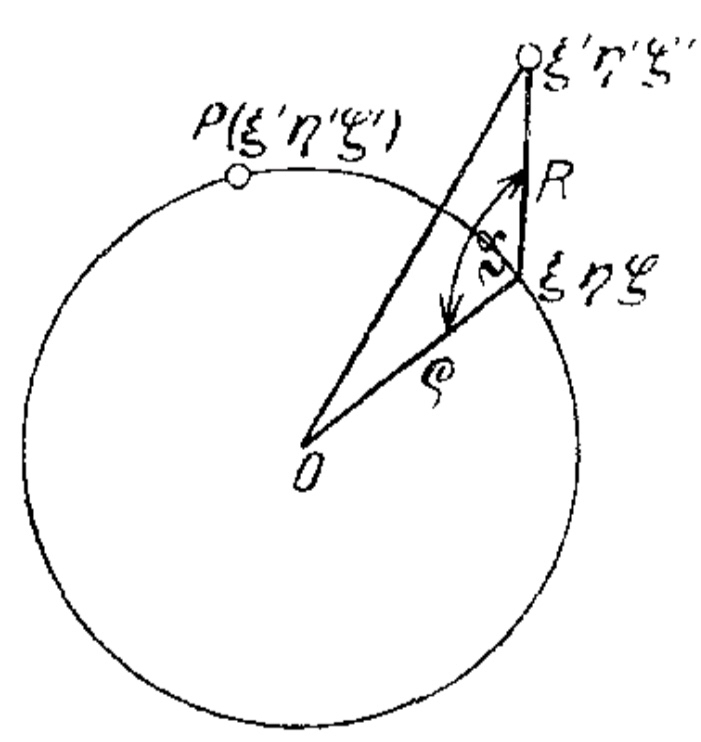
\includegraphics[width=100pt]{fig1}
\end{center}
\label{Fig. 1}
\end{figure}
by introducing instead of the quantity $R$ of (74c) the value (fig. 1) proportional to it from (52a)
\uequ{
\nu(XYZj^*) = \frac{v_{j^*}}{2\pi a}R.
}
The the plane $\varphi=0$ runs parallel to the $\zeta$-axis. Then, at fixed $\xi,\eta,\zeta$, $f(\xi'\eta'\zeta')$ depends only on $\nu,\vartheta,\varphi$. We then write $f(\xi'\eta'\zeta')=f(\nu\vartheta\varphi)$. If we note that, according to (64a)
\uequ{
\left|J_{klm,k'l'm',1}\right|^2=\frac{C^2}{4\mu^2 a^2}R^2 = \frac{\pi^2 C^2}{\mu^2 v^2}\nu^2(XYZ,1),
}
we obtain
\uequ{
n_a= \frac{G^3}{8\pi^3}\frac{2\pi^2 C^2}{\mu^2 v^2}\frac{h}{8\pi^2 M}
\cdot\left(\frac{2\pi a}{v}\right)^3 \dX{}\dY{t}\iiint\nu^3\sin\vartheta\d\nu\,\d\vartheta\,\d\vartheta\\
\cdot\sum\limits_{q(\nu\vartheta\varphi)=0}^\infty g\left[q(\nu\vartheta\varphi)\right]\\
\cdot\left\{f(\xi\eta\zeta)\left[1-f(\nu\vartheta\varphi)\right]\left[
q(\nu\vartheta\varphi)\Omega(E-E'+h\nu)\right.\right.\\
\left.\left.\left[q(\nu\vartheta\varphi)+1\right]\cdot\Omega(E-E'+h\nu)\right]\right.\\
\left. - f(\nu\vartheta\varphi)\left[1-f(\xi\eta\zeta)\right]\left[
q(\nu\vartheta\varphi) \Omega(E-E'+h\nu)\right.\right.\\
\left.\left.\left[q(\nu\vartheta\varphi) +1\right] \Omega(E-E'+h\nu)
\right]\right\}.
}
Now according to (63c) $E=\omega\varrho^2$, hence (cf fig. 1)
\uequ{
E-E' = \omega(R^2-2\varrho R\cos\vartheta).
}
If in place of $\vartheta$ we introduce
\uequ{
y=E-E'\pm h\nu = \omega\left(\frac{4\pi^2 a^2}{v^2}\nu^2 - 2\varrho\frac{2\pi a}{v}\nu\cos\vartheta\right)\pm h\nu,
}
then
\uequ{
\nu\sin\vartheta = \frac{v}{4\pi\varrho a\omega}\d{y}
}
and integrating over $\vartheta$ in (75) we obtain expressions of the form
\uequ{
\int\Omega(y)dy = \int\frac{1-\cos\frac{2\pi t}{h}y}{y^2}\d{y}.
}
If $t$ is sufficiently large, then with the notation $x=\frac{2\pi t}{h}y$ the integral
\uequ{
\frac{h}{2\pi t}\int\Omega(y)\d{y} = \int{1-\cos{x}}{x^2}\dx
}
can be taken from $-\infty$ to $+\infty$, and it only supplies an essential contribution only in the vicinity of the pount
\uequ{
y=0,\text{i.e.} E-E' = \pm h\nu.
}
Hence one obtains
\uequ{
\int\Omega(y)\d{y} = \frac{2\pi^2}{h}.
}
\newcommand{\xiyz}{\xi\eta\zeta}
\newcommand{\noy}{\nu\vartheta\varphi}
So, from (75),
\uequ{
n_a = &\frac{(aG)^3}{M}\frac{\pi C^2}{8\varrho a\omega v^4 \mu^2}
\iint\nu^2 \d\nu\,\d\varphi \cdot\sum\limits_{q(\noy)=0}^\infty g\left[q(\xiyz)\right]\\
\left\{\right.&f(\xiyz)\left[1-f(\noy)_{E'=E+h\nu}\right]q(\noy)\\
+&f(\xiyz)\left[1-f(\noy)_{E'=E-h\nu}\right]\left[q(\noy)+1\right]\\
-&f(\noy)_{E'=E-h\nu}\left[1-f(\xiyz)\right]q(\noy)\\
-& \left.f(\noy)_{E'=E+h\nu}\left[1-f(\xiyz)\right]\left[q(\noy)+1\right]
\right\}
}
Inserting here the expressions (70) and (73) for $f$ and $g$,
\uequ{
n_a = &\frac{(aG)^3}{M}\frac{\pi C^2}{8\varrho a\omega v^4 \mu^2}
\iint\nu^2 \d\nu\,\d\varphi \cdot\sum\limits_{q(\nu)=1}^\infty q(\nu)\cdot\exp{-\frac{qh\nu}{kT}}\left(1-\exp{-\frac{h\nu}{kT}}\right)\\
\left\{\vphantom{\xi}\right.
&\left[f_0(E) + \xi\chi(E)\right]\left[1-f_0(E+h\nu)-\xi'\chi(E+h\nu)\right]\\
+&\left[f_0(E) + \xi\chi(E)\right]\left[1-f_0(E-h\nu)-\xi'\chi(E-h\nu)\right]\exp{\frac{h\nu}{kT}}\\
-&\left[f_0(E-h\nu)+\xi'\chi(E-h\nu)\right]\left[1-f_0(E)-\xi\chi(E)\right]\\
-&\left.\left[f_0(E+h\nu)+\xi'\chi(E+h\nu)\right]\left[1-f_0(E)-\xi\chi(E)\right]\cdot\exp{\frac{h\nu}{kT}}\right\}.
}
The $\chi$-free terms vanish, e.g.
\uequ{
f_0(E)\left[1-f_0(E+h\nu)\right] - \exp{\frac{h\nu}{kT}}\cdot f_0(E+h\nu)\left[1-f_0(E)\right]=0\\
}
or by (69),
\uequ{
\exp{\frac{h\nu}{kT}}\frac{1-f_0(E)}{f_0(E)} =
\frac{1-f_0(E+h\nu)}{f_0(E+h\nu)} = \frac{\exp{\frac{E+h\nu}{kT}}}{A}.
}
Further,
\uequ{
\sum\limits_{q(\nu)=1}^\infty q(\nu)\cdot\exp{-\frac{qh\nu}{kT}}
\left(1-\exp{-\frac{h\nu}{kT}}\right) = \frac{1}{\exp{\frac{h\nu}{kT}}-1}.
}
Neglecting the terms quadratic in $\chi$, then after repeated usage of the formula (69), and noticing that by interaction with the $b$-oscillators the same expression again occurs, i.e. \?{there is an additional factor of 2}{ein Faktor 2 dazu kommt}
\nequ{76}{
n_a = & \frac{(aG)^3}{M}\frac{2\pi C^2}{8\varrho a\omega v^4 \mu^2}
\iint\frac{\nu^2\d\nu\varphi}{\exp{\frac{h\nu}{kT}-1}}\left\{
\xi\chi(E)\frac{f_0(E+h\nu)\cdot\exp{h\nu}{kT}+f_0(E-h\nu)}{f_0(E)}\right.\\
-  &\left.\xi'\left[\chi(E+h\nu)\frac{f_0(E)}{f_0(E+h\nu)}
+ \chi(E-h\nu)\frac{f_0(E)\cdot\exp{\frac{h\nu}{kT}}}{f_0(E-h\nu)}
\right]
\right\}.
}
Now static equilibrium shall reign in the presence of a field, i.e. according to (50) and (74c) we must have
\uequ{
n_a=-\frac{2\pi eFa}{h}\pX{f_0}\pY{\xi}=-\frac{\pi eFa}{h}\pX{f_0}\pY{\varrho}\frac{\xi}{\varrho}.
}
As in the theory of the specific heats of solid bodies we cut off the elastic spectrum at a limiting frequency $\nu_g$ which is given by $\frac{h\nu_g}{k\Theta}=1$, where $\Theta$ denotes the characteristic temperature of the body. Introducing $x=\frac{h\nu}{kT}$ as a new integration variable in (76), we get
\nequ{77}{
n_a &= \frac{G^3}{M}\cdot\frac{2\pi C^2}{8\varrho a\omega v\mu^2}\left(\frac{ak\Theta}{h\nu}\right)^3\cdot\left(\frac{T}{\Theta}\right)^3\\
\cdot\int\limits_{x=0}^{\Theta/T}\int\limits_{\varphi=0}^{2\pi}
&\frac{x^2 \dx\,\d\varphi}{\exp{x}-1}\left\{\xi\chi(E)
\frac{f_0(E+kTx)\cdot\exp{x} + f(E-kTx)}{f_0(E)}\right.\\
- &\left.\xi'\left[\chi(E+kTx)\frac{f_0(E)}{f_0(E+kTx)}
+ \chi(E-kTx)\frac{f_0(E)\cdot\exp{x}}{f_0(E-kTx)}
\right]\right\}\\
&= -\frac{2\pi eFa}{h}\dX{f_0}\dY{\varrho}\frac{\xi}{\varrho}.
}

Since the point $\xi'\eta'\zeta'$ [cf the point $P$ ($\xi'\eta'\zeta'$) in figure 1] essentially lies in a sphere about 0 with radius $\varrho$,
\uequ{
\xi' = \xi-X = \xi - \frac{\xi R^2}{2\varrho^2} - R\cos\varphi\sqrt{1-\left(\frac{R}{2\varrho}\right)^2}\sqrt{1-\left(\frac{\xi}{\varrho}\right)^2},
}
and
\uequ{
R^2 = \frac{4\pi^2 a^2}{v^2}\nu^2 = 4\pi^2\left(\frac{ak\Theta}{hv}\right)^2\left(\frac{T}{\Theta}\right)^2 x^2.
}
Inserting this into (77), the term with $\cos\varphi$ vanishes upon integration over $\varphi$, and dividing both sides by $\frac{2\pi\xi}{\varrho}$ what remains is
\nequ{78}{
&\frac{G^3}{M}\frac{2\pi C^2}{8a\omega v\mu^2}\left(\frac{ak\Theta}{hv}\right)^3\left(\frac{T}{\Theta}\right)^3
\int\limits_0^{\Theta/T}\left\{\chi(E)\frac{f_0(E+kTx)\exp{x} + f_0(E-kTx)}{f_0(E)}\right.\\
&\left. - \chi(E+kTx)\frac{f_0(E)}{f_0(E+kTx)}-\chi(E-kTx)\frac{f_0(E)\exp{x}}{f_0(E-kTx)}\right\}\frac{x^2\dx}{\exp{x}-1}\\
&\frac{1}{2\varrho^2}\frac{G^3}{M}\frac{8\pi^3 C^2}{8a\omega v\mu^2}
\left(\frac{ak\Theta}{hv}\right)^5\left(\frac{T}{\Theta}\right)^5
\int\limits_{0}^{\Theta/T}\left\{\chi(E+kTx)\frac{f_0(E)}{f_0(E+kTx)}\right.\\
&\left.+ \chi(E-kTx)\frac{f_0(E)\exp{x}}{f_0(E-kTx)}\right\}\frac{x^4\dx}{\exp{x} - 1}\\
&= -\frac{eFa}{h}\pX{f_0}\pY{\varrho} = -\frac{eFa}{h}\pX{f_0}\pY{E}2\omega\varrho.
}
\begin{figure}[h]
\begin{center}
	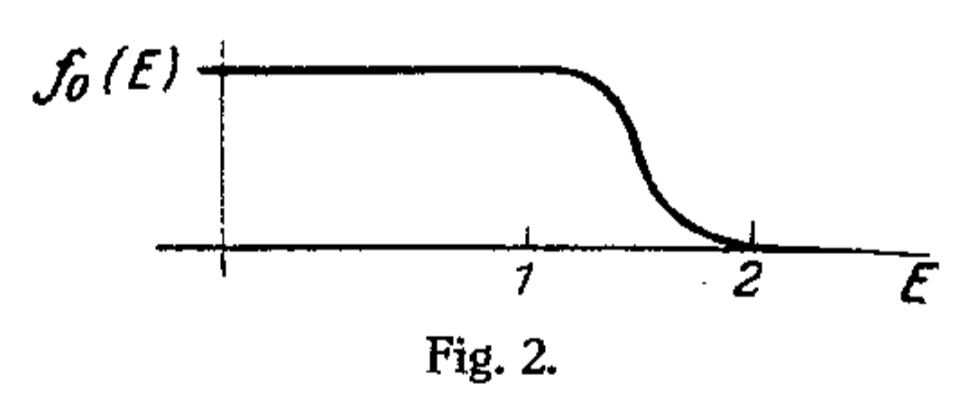
\includegraphics[width=200pt]{fig2}
\end{center}
\end{figure}

If the electron gas is completely degenerate, then in (65) one must put
\uequ{
A=\exp{\frac{\omega\varrho_0^2}{kT}},
}
where, as in \S2
\uequ{
\varrho_0=\sqrt[3]{6\pi^2 x}
}
and $\omega\varrho_0^2$ is the energy in which the drop-off of $f_0(E)$ (cf the interval 1-2 of Fig. 2). Introducing instead of $E$ the dimensionless quantity
\nequ{79}{
\varepsilon = \frac{E-\omega\varrho_0^2}{kT},
}
then 
\nequ{79a}{
f_0(E) = f_0(\varepsilon) = \frac{1}{\exp{x}+1}
}
and
\nequ{79b}{
-\pX{f_0}\pY{E} = -\frac{1}{kT}\dX{f_0}\dY{\varepsilon}
= -\frac{1}{kT}\frac{1}{(\exp{\varepsilon} + 1)(\exp{-\varepsilon}+1)}
}
will only be perceptibly different from zero in the vicinity of the point $\varepsilon=0$. Then one can replace the quantity $\varrho$ occurring in (78) by $\varrho_0$. In place of the desired function $\chi(E)=\chi(\varepsilon)$ we now introduce a new one
\nequ{80}{
c(\varepsilon) = kT(\exp{\varepsilon} + 1)(\exp{-\varepsilon} + 1)\chi(\varepsilon) = \frac{\chi(E)}{-\pX{f_0}\pY{E}}.
}
Further, if we also use the abbreviations
\nequ{81}{
P=\frac{eFa}{h}\frac{M}{G^3}\frac{16a\omega^2\varrho_0 v\mu^2}{2\pi C^2}
\left(\frac{hv}{ak\Theta}\right)^3;\quad
Q=\frac{4\pi^2}{2\varrho_0^2}\left(\frac{ak\Theta}{hv}\right)^2,
}
then, from 78, using (79a, b)
\nequ{82}{
\int\limits_0^{\Theta/T}&\left\{
\frac{\exp\varepsilon + 1}{\exp\varepsilon + \exp{-x}}\left[
c(\varepsilon) - \left(1-Q\left(\frac{T}{\Theta}\right)^2 x^2\right)c(\varepsilon + x)\right]\right.\\
&\left. + \frac{\exp{-\varepsilon} + 1}{\exp{-\varepsilon} + \exp{-x}}\left[
c(\varepsilon) - \left(1-Q\left(\frac{T}{\Theta}\right)^2 x^2\right)c(\varepsilon - x)\right]\right\}
\frac{x^2\dx}{\exp{x}-1} = P\left(\frac{\Theta}{T}\right)^3.
}

Since the electron can not give up more energy than its original value of $E$, in the last term the integral might rigorously only be taken up to the point $kTx=E$. Since however, as we will show below, we are only interested in the value of the function $c(\varepsilon)$ in the vicinity of the critical points, i.e. where $E=\omega\varrho_0^2$ and since $k\Theta<\omega\varrho_0^2$, the integration limit $\frac{\Theta}{T}$ remains valid.

We will now separately consider the temperature dependence of the conductivity for the two following cases:

1. $T\gg\Theta$. Here we expect the same results for $\chi(E)$ that Lorentz (l.c.) found according to the classical statistics, namely
\uequ{
\chi(E) = -c\pX{f_0}\pY{E},
}
where, according to (79b) and (80)
\uequ{
c(\varepsilon) = c = \text{const.}
}

The essential difference between our calculation and the classical one lies in the \?{molecular chaos assumption}{Stoßzahlansatz} satisfying the Pauli exclusion principle.  This is expressed in (72) in the bracketed expression, where in the classical calculation one would simply obtain
\uequ{
g(q)\left[f(klm)-f(k'l'm')\right].
}
But now for $T\gg\Theta$ all the \?{frequency components}{Eigenschwingungen} are strongly excited, i.e. their quantum numbers $q\gg 1$, so that $q'=q\pm 1$ may be replaced by $q$. But putting
\uequ{
g(q) = g(q')
}
in (72) one again obtains just the classical result\footnote{L.W. Nordheim, Proc. Roy. Soc. 119, 689, 1928, has given justification to the calculations by Sommerfeld and Houston on which the classical expression is based, insofar as the electron is elastically reflected by the lattice. Then would in fact always have to set $g(q)=g(q')$. Here however this is not permissible and this distinction is, as we will show in the following, essential for low temperatures.}.

In fact, equation (82) satisfies the \textit{Ansatz}
\uequ{
c(\varepsilon) = c.
}
Since $\frac{\Theta}{T}\ll 1$ and hence $x\ll 1$, one may put
\uequ{
Q\left(\frac{T}{\Theta}\right)^2\int\limits_0^{\Theta/T}\left\{
\frac{\exp{\varepsilon}+1}{\exp{\varepsilon}+\exp{-x}}c(\varepsilon+x) +
\frac{\exp{-\varepsilon}+1}{\exp{-\varepsilon}+\exp{-x}}c(\varepsilon-x) 
\right\}\frac{x^4\dx}{\exp{x}-1}\\
= 2cQ\left(\frac{T}{\Theta}\right)^2\int\limits_0^{\Theta/T}x^3\dx
= \frac{c}{2}Q\left(\frac{\Theta}{T}\right)^2
= P\left(\frac{\Theta}{T}\right)^3.
}
So according to (80)
\uequ{
\chi(E) = -c\pX{f_0}\pY{E} = -\frac{2P}{Q}\frac{\Theta}{T}\pX{f_0}\pY{E}
= -\frac{2P}{2\omega\varrho}\frac{\Theta}{T}\pX{f_0}\pY{\varrho}.
}
Replacing $\varrho$ by $\varrho_0$ back in (78) for simplification as in (82), in (81) one has to write $\varrho$ instead of $\varrho_0$ for $P$ and $Q$ (which is of course of no importance for the calculation of the conductivity) and obtains
\nequ{83}{
\chi(\varrho) = -\frac{4FeMa^2\varrho^2\omega v\mu^2}{G^3\pi^3 C^2 h}\left(\frac{hv}{ak\Theta}\right)^5 \pX{f_0}\pY{\varrho}\frac{\Theta}{T}.
}
Since according to (63d) the momentum in the $x$-direction in the $\zeta\eta\zeta$ state is $\tau\xi$, the current per $\unit{cm}^3$ in the stationary distribution (70) is given by
\nequ{84}{
J=\frac{2e}{mV}\iiint\tau\xi^2\chi(\varrho)\frac{G^3}{8\pi^3}\d\xi\,\d\eta\,\d\xi.
}
The current arising from $f_0(\xi\eta\zeta)$ vanishes and the factor 2 in (84) arises from the fact that, because of the spin, the statistical weight  of each state must be doubled. $V$ is the volume of our piece of crystal. Using the expressions (83) and (65), as well as the value found in \S3 for degenerate gasses, the further calculation runs exactly as in Sommerfeld, l.c.:
\uequ{
\log{A} = \frac{\omega}{kT}(6\pi^2\varkappa)^\frac{2}{3}.
}

Finally we obtain for the conductivity
\nequ{85}{
\sigma = \frac{J}{F} = \frac{4(6\pi^2\kappa)^2}{3\pi^5}\cdot
\frac{e^2 d\tau\,\omega v a^2\mu^2}{mC^2 h}\left(\frac{hv}{ak\Theta}\right)^5\cdot\frac{\Theta}{T},
}
$d=\frac{M}{V}$ is the density of our substance.

Next we want to estimate the magnitude of the expression obtained in (85). $\omega$ is, as in \S2, an energy of order $\beta'\cdot 10^{-12}\unit{erg}$. $\tau/m$ is according to (63d) of the same order as the maximal speed of the electron, since $k$ runs through values from $-G$ to $+G$ in (63d). For Sommerfeld's free electrons it comes to $10^8\unit{cm}\cdot\unit{sec}^{-1}$. We will put $\frac{\tau}{m}=\tau'\cdot 10^8\unit{cm}\cdot\unit{sec}^{-1}$, so that $\tau'$ as well as $\beta'$ are both of order 1 for free electrons, \?{and thereby consider the connection that we set to $\tau'=\beta'=\frac{1}{10}$}{und die Bindung dadurch ber\"ucksichtigen, da\ss wir setzen $\tau'=\beta'=\frac{1}{10}$}. According to (64) $C$ is the reciprocal square of a length on the order of an atomic radius, i.e. $10^{-8}\unit{cm}$. $\frac{hv}{ak\Theta}$ is, as one is easily convinced, a pure number of order 1. If $T=3\Theta$, then we obtain with these values $\sigma \approxeq 10^{18}$\?{electrostatic units}{elst. Einh.}. This value, in harmony with experiment, is in any case satisfactory in view of our rough assumptions.

For the resistance $W=\frac{1}{\sigma}$ we obtain the long-experimentally-known proportionality with the absolute temperature, as was also found by W.V. Houston, l.c.

2. $T\ll\Theta$: Our conductor however shows a totally different behavior at low temperatures. Without consideration of the zero-point motion of the lattice, W.V. Houston has found here a decrease proportional to $T^2$. Had the zero-point energy been taken into account, as demanded by the quantum mechanics, by applying the corresponding formula for the scattering of Roentgen rays derived by Debye and Waller\footnote{P. Debye, Ann. d. Phys. (4) 43, 49, 1914; J. Waller, ibid (4) 83, 153, 1927.}, an additional temperature-independent resistance would be had which would give at absolute zero about a fourth of the resistance at room temperature. At first it seems difficult to escape this fact that is fully in contradiction with experiment, all the more as the scattering of Roentgen rays clearly indicates the existence of a zero-point motion in agreement with theory.

We will show that nevertheless our formula (78) correctly reproduces the vanishing of the resistance at low temperatures.

This rests on the circumstance highlighted above in equation (62a), that in each scattering process the energy $h\nu$ must be taken by or given up by the lattice. The energy given up by the lattice at decreasing temperatures is always the least possible, since the lattice always contains less energy. The energy increase in the lattice is on the other hand \?{unchanged, even at the lowest temperatures}{selbst bei tiefsten Temperaturen unver\"andert m\"oglich}, and leads in general to the mentioned residual resistance at absolute zero (cf scattering of Roentgen rays). In our case however even the scattered electrons (in contrast to the just-mentioned case of Roentgen rays) are in thermal equilibrium, and therefore can give up less and less energy to the lattice at decreasing temperature. So, if at decreasing temperature the processes that in general give rise to residual resistance become increasingly rare, the residual resistance vanishes.

I have not succeeded in rigorously determining the function $c(\varepsilon)$ from the integral equation (82), which would be essential for an exact calculation of the resistance. In order to show that for low temperatures the resistance vanishes proportionally to $T^3$, it suffices to examine the asymptotic behavior of the function $c(\varepsilon)$ for $|\varepsilon|\gg 1$. The physical basis for this lies, as we shall show below, in how this begavior depends on how strongly the short-waved vibrations -- only very few of them excited at low temperatures -- are influenced by the collisions of the electrons.

We will initially assume that $c(\varepsilon)$ strongly increases for $\frac{\Theta}{T}\gg\varepsilon\gg 1$, approximately like a function $\varepsilon^n\exp{\varepsilon}$, where $n$ is any positive or negative number of order 1, \?{and this assumption leads to an \textit{ad absurdum}}{und diese Annahme ad absurdum f\"uhren}. Here we constrain ourselves to $\varepsilon>0$, since according to (82)
\uequ{
c(\varepsilon)=c(-\varepsilon).
}
From (82), for $\varepsilon\gg 1$
\nequ{86}{
P\left(\frac{\Theta}{T}\right)^3=&c(\varepsilon)\int\limits_0^{\Theta/T}
\frac{x^2\dx}{\exp{x}-1}-\int\limits_0^{\Theta/T}c(\varepsilon+x)\left[
1-Q\left(\frac{T}{\Theta}\right)^2 x^2\right]\frac{x^2\dx}{\exp{x}-1}\\
+&c(\varepsilon)\int\limits_0^{\Theta/T}\frac{x^2\dx}{(\exp{x}-1)(\exp{-\varepsilon}+\exp{-x})}\\
-&\int\limits_0^{\Theta/T}c(\varepsilon-x)\left[1-Q\left(\frac{T}{\Theta}\right)^2 x^2\right]\frac{x^2\dx}{(\exp{x}-1)(\exp{-\varepsilon}+\exp{-x})}.
}
The third summand may be replaced by $c(\varepsilon)\int\limits_0^\varepsilon x^2\dx = \frac{\varepsilon^3}{3}c(\varepsilon)$, since the integrand may be replaced by $x^2$ for $1\ll<\varepsilon; \exp{-x}\gg\exp{-\varepsilon}$, where it gives its primary contribution, and vanishes exponentially for $x>\varepsilon$ as soon as $\exp{-x}\ll\exp{-\varepsilon}$. The fourth summand may be ignored, since for the essential part $1\ll x<\varepsilon$
according to our assumption $c(\varepsilon-x)\ll c(\varepsilon)$ and since for $x>2\varepsilon$, where (since $c(\varepsilon)$ is an even function) $c(\varepsilon-x)=c(\varepsilon)$ or even $c(\varepsilon-x)\gg c(\varepsilon)$ the $\exp{x}$ in the denominator ensures that there the fourth summand can be ignored compared to the second. The integral in the first summand is a number of order 1, may then be ignored compared to the $\frac{\varepsilon^3}{3}\gg 1$ and instead of (86) one may write
\uequ{
P\left(\frac{\Theta}{T}\right)^3 = \frac{\varepsilon^3}{3}c(\varepsilon) - \int\limits_0^{\Theta/T}c(\varepsilon+x)\left[
1-Q\left(\frac{T}{\Theta}\right)^2 x^2\right]\frac{x^2\dx}{\exp{x}-1}.
}
This integral equation however will be solved for $\varepsilon\gg 1$ by the \textit{Ansatz}
\uequ{
c(\varepsilon)=\frac{3P}{\varepsilon^2}\left(\frac{\Theta}{T}\right)^3,
}
since then the integral vanishes for increasing values of $\varepsilon$, and hence the assumption of a $c(\varepsilon)$ increasing exponentially for great values of $\varepsilon$ is refuted as self-contradictory.

Then it follows that
\uequ{
\chi(\varepsilon) = \frac{c(\varepsilon)}{kT(\exp{\varepsilon}+1)(\exp{-\varepsilon}+1)},\text{ for } |\varepsilon|\gg 1
}
exponentially vanishes because of the increase of the denominator, since this cannot be compensated by a corresponding increase of $c(\varepsilon)$. This means that only those electrons contribute noticeably to the conduction current whose energy lies at the critical points from 1 to 2 (figure 2).

But if $\varepsilon$ is of order 1, then (82) does not change essentially if instead of $\frac{\Theta}{T}\gg 1$, $\infty$ is set for the upper limit, since for $x\gg 1$, $c(\varepsilon-x)$ and $c(\varepsilon+x)$ cannot increase to the extent needed to prevent the integral from vanishing because of the $\exp{x}$ in the denominator. So it is said that those vibrations for whose frequency the relation $x=\frac{h\nu}{kT}\gg 1$ applies no longer play an essential role in the formation of the resistance, i.e. only longer-waved modes participate, the lower the temperature. Since $Q$ is a pure number of order 1, in (82) $Q\left(\frac{T}{\Theta}\right)^2 x^2$ may be neglected compared to 1 and for a given $\varepsilon$, thanks to the $\left(\frac{\Theta}{T}\right)^3$ on the left side, $c(\varepsilon)$ only depends on the temperature, i.e.
\uequ{
c(\varepsilon) = \left(\frac{\Theta}{T}\right)^3 c^*(\varepsilon),
}
where $c^*(\varepsilon)$ now only depends on $\varepsilon$ alone. From that it follows according to (80) that in the vicinity of the critical points:
\uequ{
\chi(E) = -\pX{f_0}\pY{E}\left(\frac{\Theta}{T}\right)^3 c^*\left(\frac{E-\omega\varrho_0^2}{KT}\right),
}
and hence as in (84) the current is
\uequ{
J=\frac{2e\tau}{mV}\iiint\xi^2\chi(\varrho)\frac{G^3}{8\pi^3}\d\xi\,\d\eta\,\d\zeta = \frac{4\pi}{3\omega}\cdot
\frac{e\tau}{mV}\frac{G^3}{8\pi^3}\left(\frac{\Theta}{T}\right)^3 6\pi^2 \varkappa\cdot c^*(0),
}
and therefore for the resistance
\uequ{
W\approx T^3.
}
The empirical formula put forward by Gr\"uneisen\footnote{See e.g. Handb. d. Phys. XIII, p.18.} demands $W\approx T^4$, yet newer measurements seem to also justify the $T^3$-law.

It is absolutely essential that the "collisions" of the electrons with the lattice are completely elastic, rather than being accompanied by an energy exchange. The former is of course based on the heating of the conductor through which a current flows. But then this fact is as mentioned above also decisive for the vanishing of the resistance with the temperature. If one simply puts $E\pm h\nu$ in (76) instead of $E$, then one obtains a law for the resistance of the form
\uequ{
W\approx\left(\frac{T}{\Theta}\right)^5\cdot\int\limits_0^{\Theta/T}
\frac{\exp{x}+1}{\exp{x}-1}x^4 \dx
 = 2\left(\frac{T}{\Theta}\right)^5\cdot\int\limits_0^{\Theta/T}\frac{x^4\dx}{\exp{x}-1}+\frac{1}{5},
}
i.e. an additional temperature-dependent resistance, as would also be found according the theory of head radiation of Roentgen rays by considering he zero-point motion of the lattice.

In \S3 it was shown that degenerate and non-degenerate gasses show entirely different behavior as regards their specific heats. We will show that this also applies for electrical conductivity, by examining alongside the just-treated $\gamma\gg 1$ case of degenerate gasses, the case $\gamma\ll 1$.

The considerations run essentially the same way as with $\gamma\gg 1$. One again obtains
\nequ{87}{
\chi(\varrho) = -c(\varrho)\pX{f_0}\pY{\varrho}.
}
We expand $f_0$ in powers of $1/T$ as in (33) and indeed with (63c) one obtains
\uequ{
f_0=&\frac{A}{A+1}\left[1-\frac{1}{A+1}\left(\frac{\omega}{kT}\varrho^2 + \dots\right)\right],\\
&\pX{f_0}\pY{\varrho} = -2\varrho\frac{\omega}{kT}\frac{A}{(A+1)^2}.
}
Inserting this into (87) and calculating the current and from that the resistance as in (84), again using the temperature $T_0=\frac{\omega}{k}$ which we will suppose $T_0\ll\Theta$, one obtains for $T\ll T\ll\Theta$ as a consequence of the zero-point motion
\uequ{
W\approx T
}
and for $T_0\ll\Theta\ll T$
\uequ{
W\approx T^2,
}
though the latter law would never be found in conductors. With the last consideration we will only show that the possibility exists of a transition between two totally different laws for conductivity, which takes place at one of the characteristic, fully independent temperatures. That such transitions actually occur is shown by the phenomenon of superconductivity, which however has still yet to be explained.

To close I would like to express my most heartfelt thanks to Herrn Professor Heisenberg for the impetus for this work as well as for his continual interest in its progress and the numerous valuable consultations that he let me take part in.

Leipzig; Institut d. Universit\"at f. theor. Physik, June 25th, 1928.


\end{paper}